% !TEX root = ../These_Robin_Master.tex
\setcounter{chapter}{0}
\graphicspath{{chap1/}}


\chapter{Modélisation et visualisation à l'interface entre les disciplines}
\label{chap:chap1}
\vspace*{-3.5em}
\begin{center}
	{\large Version \hl{2019-12-16}}
\end{center}
\vspace*{-2.5em}
\begin{itemize}
	\item 10/10/2019 : Nouveau plan
	\item 22/10/2019 : fin écriture + relecture + rendu Lena
	\item 18/11/2019 : fin reprise + ajouts (reproductibilité + intro + ccl)
	\item 06/12/2019 : fin reprise + envoi relecture externe Julien
	\item 16/12/2019 : reprise commentaires Julien\footnote{
	Manque : p. 2, 	26, 41
} + envoi Clarisse
\end{itemize}%\vspace*{-1.5em}
\vspace*{-1.5em}
\setcounter{minitocdepth}{2}
\minitoc
\clearpage
\phantomsection

\section*{Introduction}
\addcontentsline{toc}{section}{\protect\numberline{}Introduction}

Le travail de thèse présenté dans ce manuscrit est hybride, et donc peu évident à positionner dans l'espace des disciplines académiques, tant l'objet décrit (la modélisation de dynamiques spatiales), le cas d'étude (l'évolution du système de peuplement rural en Touraine entre les IX$^e$ et XIII$^e$ siècles) et la méthode mise en place (la simulation multi-agents) semblent relever de disciplines différentes (géographie, sciences historiques et informatique).

Cet aspect pluridisciplinaire complexifie la structure démonstrative classique d'une thèse en géographie, et il me paraît\footnote{
	Dans ce chapitre, très personnel et consacré essentiellement à la description et justification d'un positionnement individuel, le choix de la première personne du singulier me semble tout à fait adapté.
	Dans le reste de ce manuscrit, qui s'inscrit dans un contexte collectif dont plusieurs dimensions sont elles aussi collectives, la première personne du pluriel sera exclusivement mobilisée.
} dès lors inadapté d'engager cette argumentation par l'habituel état de l'art, celui-ci ne pouvant être cantonné à un unique sujet dans ce travail.

Au contraire, je crois que ce premier chapitre offre plutôt l'occasion de clarifier, en l'explicitant, la position de ce travail universitaire, et plus globalement, des recherches menées dans le cadre de cette thèse.
Ce manuscrit et les productions informatiques qui l'accompagnent\footnote{
	La forme numérique de ces productions, organisée dans des dépôts logiciels qui sont systématiquement communiqués dans cette thèse, me paraît plus adaptée qu'une reproduction dans le manuscrit.
} ne visent pas à approfondir un questionnement thématique précis, mais s'ancrent à l'inverse dans une position assumée et engagée de démarche méthodologique.
C'est dans ce sens que ce manuscrit devrait être compris, en considérant que les solutions mises en œuvre pour l'analyse d'un cas d'étude particulier ont en réalité une vocation de généricité et de reproductibilité.
L'apport majeur de ce travail se veut ainsi méthodologique, et c'est à ce titre qu'il s'inscrit à l'interface entre plusieurs disciplines, mobilisant des connaissances et méthodes de chacune.

Dans ce chapitre, je tiens à expliciter le positionnement de ce travail méthodologique, à l'interface entre la géographie, l'informatique et les sciences historiques et des approches méthodologiques plurielles.
Pour expliciter cette position et l'engagement collectif qui la définit, il m'apparaît nécessaire d'en décrire la genèse au travers  (1) de mon parcours personnel et (2) du contexte de conception de cette thèse.
La description (3) du questionnement qui en résulte et de son évolution dans le contexte de ce travail de recherche, permettront enfin (4) de justifier l'approche suivie tout au long de cette expérience, sous une forme programmatique engagée.


\section{Parcours scientifique et professionnel : vers la modélisation en géographie \label{sec:formation}}

Le travail de recherche présenté dans cette thèse s'inscrit profondément à l'interface entre plusieurs courants disciplinaires liés à l'étude des phénomènes sociaux dans l'espace.
Pour en comprendre aussi bien le questionnement que l'approche mobilisée et les résultats obtenus, il me paraît important de faire un rapide retour sur ma formation initiale et début de parcours dans le monde de la recherche académique, qui explique et préfigure assez largement le positionnement adopté dans ce travail.
Depuis une formation classique de géographie humaine et urbaine jusqu'à l'exercice de fonctions d'ingénieur d'étude en modélisation, en passant par une spécialisation en géomatique et cartographie, chacune des étapes de ma formation permet de mieux comprendre la formulation de l'aboutissement de cette thèse fondée sur la co-construction interdisciplinaire de modèles spatiaux et sur leur exploration graphique.

\subsection{Géographie}

Ce travail de recherche s'inscrit avant tout, tant administrativement que conceptuellement, dans le champ disciplinaire de la géographie.
Cette discipline, consacrée à l'étude de la dimension spatiale de phénomènes sociaux, constitue les fondements de ma formation initiale.
En sortant de classes préparatoires littéraires généralistes, j'avais ainsi été frappé par l'exercice du commentaire de cartes, à visée tant verticale (cartes géologiques) qu'horizontale (cartes topographiques).
On pouvait décrire et expliquer le fonctionnement économique et social d'un lieu par la seule observation de ses structures et de ses contextes spatiaux.

\paragraph{Géographie urbaine.}

Cela m'a mené vers un cursus universitaire classique de géographie, majoritairement marqué par la géographie humaine et l'étude de grandes tendances spatiales dans les interactions sociales humaines.
Avec un intérêt pour l'aménagement et l'urbanisme, la géographie urbaine, dans sa dimension sociale, m'est rapidement apparue comme particulièrement stimulante dans sa capacité à décrypter, à expliquer et à comparer des processus sociaux variés à l'échelle intra-urbaine.
Il ne s'agissait plus simplement de décrire un état, mais d'en expliquer les processus spatiaux et sociaux.
Au regard des enseignements d'urbanisme et de politiques de la ville, ces approches permettaient ainsi de comparer le résultat de différentes politiques publiques, et de mener un début de mesure de l'écart entre leur objectif exprimé et leur action effective.

En master, j'ai voulu appliquer ces approches en initiant, sous la co-direction de Renaud Le Goix et Antonine Ribardière, un mémoire sur la comparaison de l'intégration spatiale des migrants entre les politiques francophones et anglophones.
Les politiques migratoires francophones, nourries du modèle jacobin français, menaient-elles à une plus forte inclusion et mixité sociale que les modèles anglophones, fondés sur l'image d'un \og \textit{salad-bowl}\fg{} communautaire ?
Le cas d'étude choisi portait sur le Canada, pays ayant l'avantage de présenter ces deux communautés linguistiques et culturelles -- francophones jacobines et anglophones communautaires --, et d'avoir une forte culture -- et attractivité -- migratoire, aussi bien pour les pays les plus développés que pour les Suds.
Le recensement canadien, enfin, permettait les études ethniques et communautaires en offrant des statistiques ethniques rares dans les autres pays.

\paragraph{Géographie Théorique et Quantitative.}

Dans un contexte de découverte de l'analyse spatiale, de la modélisation graphique, des systèmes d'information géographiques (SIG) et d'approches plus systémiques et horizontales de description et d'explication de phénomènes socio-spatiaux, ce travail de Master s'est assez rapidement orienté vers une démarche quantitative et à visée plus généralisante.
Le mémoire qui en a résulté, intitulé \og Ségrégation spatiale et origines ethniques dans les métropoles canadiennes\fg{}, constitue ainsi un tournant vers la géographie théorique et quantitative (GTQ).
L'approche, très quantifiée, fait la part belle à la comparaison des différents indices de ségrégation caractérisant les distributions spatiales de la population urbaine canadienne.
Pour être en mesure de mener cette comparaison de manière systématique, une auto-formation poussée avait été nécessaire, notamment sur les techniques d'analyse de données, de réduction de dimensionnalité (les recensements canadiens contiennent des centaines de catégories qui ne pouvaient toutes être traitées individuellement) et sur une première approche d'automatisation de traitements (via SAS).
Il fallait être en mesure de tester rapidement différentes hypothèses sur les quelques milliers de \og secteurs de recensement\fg{} impliqués dans l'étude.

Du point de vue méthodologique, cette première expérience d'exploration systématique d'un jeu de données m'avait montré la nécessité de parvenir à une certaine automatisation de la chaîne de traitement, depuis la sélection des données, le calcul de tel ou tel indice, jusqu'à leur représentation (carto)graphique.
Les données analysées étaient en effet hétérogènes, multidimensionnelles, et je cherchais à les caractériser par le calcul d'une dizaines d'indices de ségrégation, globaux et locaux.
Les quelques macros SAS mises en place ne permettaient alors pas une automatisation totale de cette démarche d'analyse, et les mois d'été passés aux traitements systématiques et répétitifs nécessaires à une approche comparative ne rendaient que plus criant le besoin d'une méthode intégrée et automatisée.

\subsection{Géomatique}

Après ce constat méthodologique, je me suis orienté, pour le master 2, vers une spécialisation en géomatique et cartographie, en intégrant le master professionnel Carthagéo.
Les connaissances acquises, méthodologiques et techniques, ont toutes concouru aux démarches mises en place dans ce travail de thèse.

\paragraph{Programmation, automatisation et interfaces graphiques.}

En premier lieu, Carthagéo m'a permis de découvrir des méthodes d'automatisation de chaînes de traitement de données spatiales.
Avec l'initiation à la programmation, il devenait important d'acquérir une vision algorithmique, systématique et processuelle des analyses que je menais jusque-là de manière manuelle et répétitive.
Par exemple, les successions de classifications ascendantes hiérarchiques (CAH) menées sur les données canadiennes, réalisées pour chaque métropole, pour chaque origine ethnique, et à plusieurs niveaux d'agrégation spatiale, pouvaient être automatisés une fois la démarche précisément explicitée.
En préalable à l'automatisation d'une démarche, il fallait avant tout pouvoir la formaliser, sur papier d'abord, de manière à pouvoir en réaliser une implémentation informatique dans un second temps.
C'est, pour moi, la découverte de la conception de modèles graphiques, non plus dédiés à la description d'un lieu comme dans la chorématique que j'avais découverte les années précédentes, mais à l'explicitation d'un processus d'analyse.
Avec l'automatisation permise par l'implémentation de ces chaînes de traitement, il devenait possible de mener des études systématiques, reproductibles et paramétrables.

Dans le cadre d'un projet de programmation en systèmes d'informations géographiques (SIG), j'ai aussi dû réaliser un outil -- un \textit{plugin} SIG\footnote{
	Les \textit{plugins} sont des extensions logicielles, qui ajoutent des fonctionnalités absentes à des logiciels génériques.
} --, permettant une comparaison visuelle et mesurée de la qualité de différents services de géocodage.
Ce projet, réalisé au sein de l'École Nationale des Sciences Géographiques, institution gérée par l'Institut Géographique National (IGN\footnote{
	L'IGN a depuis été renommé en \og Institut National de l'information géographique et forestière\fg{}.
}), visait notamment à comparer le géocodage proposé par une société internationale -- Google Maps -- et par un service public national -- l'IGN et la BD TOPO --.
En dehors de l'aspect technique, cette première expérience de projet de programmation appliqué a surtout été l'occasion de réfléchir à des questions d'interface homme-machine.
Comment rendre intuitif, pour un utilisateur n'ayant pas participé à sa conception, l'usage d'un outil interactif pensé pour vérifier la cohérence de géocodage de différentes adresses tirées de manière aléatoire dans l'espace francilien ?
Fallait-il privilégier la présentation de l'indicateur quantitatif  -- la distance entre les points issus du géocodage -- ou plutôt donner une idée plus contextuelle de la localisation spécifique des résultats du géocodage ?
%Paradoxalement, cet apprentissage de la programmation et de l'automatisation débouchait sur des questionnements relatifs au développement et à l'usage d'une interface graphique.
Cette sensibilité à l'\og usabilité\fg{}\footnote{
	L'usabilité est définie selon le standard \textcite{iso20189241} comme la combinaison de trois propriétés que sont \og l'efficacité\fg{} d'une interface (précision et qualité des résultats obtenus en l'employant), son \og efficience\fg{} (coût temporel et concentration que cela demande à l'utilisateur) et la satisfaction éprouvée par l'utilisateur suite à son usage \autocite[39]{zheng_interactive_2019}.
} d'un logiciel a été fondatrice pour mes travaux ultérieurs, et structure largement le présent travail de thèse (voir \hl{chapitre 5, section 5.4}).

\paragraph{Approches géométriques.}

Une autre approche mobilisée dans cette thèse est la vision processuelle \og géométrique\fg{} des traitements de données spatiales.
Dans ce type d'approches, caractérisées par le recours aux opérateurs spatiaux, les agrégations, extractions et filtrages de données sont réalisés de manières surtout spatiales plutôt qu'attributaires.
Par exemple, plutôt que de définir des voisinages comme la co-appartenance à une même structure territoriale (les communes d'un département par exemple), on aura plutôt tendance à définir ces voisinages à partir de contiguïtés spatiales d'ordre \textit{n}.
De la même manière, pour confondre des maillages différents (bureaux de vote et IRIS par exemple), on peut procéder à une agrégation au niveau administratif supérieur (la commune), mais aussi effectuer une intersection géométrique et re-ventiler les populations dans le maillage résultant.

Il s'agit ainsi de prendre en compte le contexte spatial, topologique, pour réaliser les opérations sur les données.
En somme, cela revient à mobiliser la dimension spatiale des données dans les différentes chaînes de traitement mises en œuvre, et la différencier fortement des autres dimensions, attributaires.
Ces approches sont nécessaires à la réalisation d'analyses portant sur des données de différentes granularités, de différents maillages : elles permettent en effet d'homogénéiser des informations dont la dimension spatiale est primordiale.
En tant que telle, cette vision \og géométrique\fg{} nous a été fortement recommandée et transmise dans le cadre d'enseignements en analyse spatiale.

Dans le modèle présenté dans cette thèse (\hl{chap2}), une large partie des mécanismes est caractérisé par des processus géométriques, qu'il s'agisse de la mise en place de zones tampons autour d'agrégats ou de pôles, de prises en compte du voisinage -- définition des agrégats --, de logiques de distances euclidiennes -- satisfaction de protection dépendant de la distance au château --, d'intersections et unions spatiales -- héritage des agrégats --, etc.
L'influence de mon parcours semble indéniable sur ces choix de modélisation où l'espace est traité de manière continue, démarche assez peu répandue dans les modèles de dynamiques spatiales.

\paragraph{Représentations (carto)graphiques.}

Un dernier point lié à mon enseignement de master a largement infusé sur les choix de ce travail de thèse.
Le master Carthagéo est une formation en grande partie dédiée à la cartographie, c'est-à-dire à l'apprentissage des \og règles\fg{} de représentation cartographiques et à une certaine réflexivité sur les différents messages qu'une carte peut convoyer.
La réflexion méthodologique sur les usages de la représentation (carto)graphique pour rendre compte d'un jeu de données est fortement présente dans l'ensemble des projets qui doivent être réalisés au cours de l'année de formation.
Les choix de représentation graphiques, très présents dans ce travail de thèse, ont ainsi durablement percolé depuis cet apprentissage.

\subsection{Modélisation : à la confluence de la GTQ et de la géomatique}

Master professionel oblige, la validation de Carthagéo impliquait la réalisation d'un stage de fin d'étude, en entreprise ou en unité de recherche.
J'ai eu la chance d'entamer un stage dans l'UMR Géographie-cités, en mai 2011, sous la co-direction de Thomas Louail, Clara Schmitt et Sébastien Rey-Coyrehourcq.
Ce stage, finalement intitulé \og Conception de modèles et d'outils de géosimulation \fg{} \autocite{cura_conception_2011}, était déjà organisé autour de tâches qui résonnent fortement vis-à-vis du contenu de la thèse.

Il s'agissait, de \og prendre part à toutes les étapes de la modélisation\fg{} \autocite{cura_conception_2011}, par :
\begin{compactenum}\vspace*{-.5em}
\item l'enrichissement d'un modèle de simulation (SimpopLocal) ;
\item la participation à la conception et à l'implémentation d'un second modèle de simulation (SimpopNet) ;
\item la création d'un outil de production de rapports de simulations (TrajPop) ;
\item la création d'un outil d'exploration cartographique des résultats de simulation \autocite[12-13]{cura_conception_2011}.
\end{compactenum}\vspace*{-.5em}
Ce stage de six mois, et les deux années de contrats d'ingénieur d'étude qui l'ont suivi pour en prolonger les recherches (au sein des projets GeoDiverCity, MIRO2 puis TransMonDyn)\footnote{
	Respectivement portés par Denise Pumain (ERC GeoDiverCity), Arnaud Banos (ANR MIRO2) et Lena Sanders (ANR TransMonDyn).
} ont durablement marqué mon rapport à la modélisation, à l'utilité de ses méthodes et à la manière de construire un modèle de façon collective.

\paragraph{Découverte de la modélisation à base d'agents.}

Ce stage a marqué ma découverte du domaine de la modélisation, et en particulier de la modélisation à base d'agents.
Par coïncidence, le premier modèle que j'ai eu à comprendre et à enrichir était un modèle de simulation de l'émergence et de la hiérarchisation d'un système de peuplement sur le temps long, au néolithique : SimpopLocal \autocite{schmitt_modelisation_2014,rey-coyrehourcq_plateforme_2015}.
Il s'agissait de tester des hypothèses issues de la géographie théorique et quantitative en les éprouvant, \textit{in silico}, à l'aide d'un outil informatique permettant de simuler des dynamiques spatiales.

Pour que je parvienne à comprendre et à m'approprier le modèle, mes encadrants m'avaient demandé d'ajouter un mécanisme exogène de perturbation du système simulé, afin de prendre en compte l'effet d'incidences de catastrophes naturelles. 
L'idée de mon implication était de me permettre de me former, par la pratique, aux notions sous-jacentes de la modélisation de systèmes complexes : émergence, interactions entre agents, processus endogènes et exogènes, etc.

Ces éléments ont été mis en pratique dans la participation à la conception et à l'implémentation d'un second modèle de simulation, \og SimpopNet-Réseaux\fg{}, \og modèle-jouet\fg{} servant de prototype pour le modèle SimpopNet développé plus tard \autocite{schmitt_modelisation_2014}.
Il s'agissait cette fois-ci de modéliser la co-évolution entre systèmes de villes et réseaux de communication, en simulant des potentiels d'interactions entre villes par l'intermédiaire de réseaux routiers formalisés par des graphes.

\paragraph{Visualisation et évaluation de modèle.}

Pour rendre compte de ces deux modèles -- SimpopLocal et SimpopNet --, il m'avait été demandé de développer des outils de visualisation et d'exploration de leurs comportements.
Les outils de visualisation intégrés à la plateforme de modélisation, NetLogo, n'étaient en effet pas suffisants pour rendre compte des différentes dynamiques produites par ces modèles.
Dans un premier temps, pour étudier l'effet des perturbations sur SimpopLocal, j'ai implémenté un type de représentation utilisé pour montrer l'évolution des rangs des villes d'un système, en m'appuyant sur les \og rank clocks\fg{} de \textcite{batty_rank_2006}.
Cette visualisation d'une itération à la suivante était très adaptée, mais ne permettait d'évaluer qu'une unique dimension (la stabilité des rangs) des phénomènes modélisés.
De plus, il était nécessaire de re-générer manuellement ces graphiques à chaque nouvelle sortie du modèle.

C'est par le biais de la recherche d'automatisation et de proposition de plusieurs modes de représentation que j'ai été amené à découvrir le langage R et ses possibilités de création de rapports automatiquement produits à partir de jeux de données.
L'outil qui en a découlé, intitulé TrajPop (analyse des trajectoires de population), a été en premier lieu mobilisé pour catégoriser et représenter les populations simulées de SimpopLocal.
Cela marquait ainsi un premier pas vers une évaluation systématique des sorties de simulation, permettant en outre d'archiver de manière systématisée les résultats de simulation.
Par la suite, TrajPop a été employé et amélioré pendant plusieurs années pour caractériser l'évolution des populations de systèmes de villes empiriques et non plus simulés (par exemple dans \textcite{pumain_multilevel_2015}).

\paragraph{Accompagnement à la modélisation.}

Un dernier aspect hérité de mes années de stagiaire/ingénieur d'étude à l'UMR Géographie-cités concerne un mode particulier de modélisation, pleinement inscrit dans le travail collectif.
Il s'agit d'une approche collective, collaborative voire accompagnatrice de la modélisation.
En effet, si les modèles SimpopLocal et SimpopNet étaient pilotés par des doctorants-modélisateurs, j'ai aussi participé à une expérience de modélisation commune où mon rôle, mi-modélisateur mi-accompagnateur, consistait à formaliser et implémenter des hypothèses sur la constitution de réseaux de collaboration scientifique.
Marie-Noëlle Comin, géographe qui avait réalisé une thèse empirique sur le sujet \autocite{comin_reseaux_2009}, cherchait ainsi à tester différents scénarios explicatifs aux regroupements de chercheurs dans le cadre de la constitution de consortiums en vue de candidature à des financements de projets scientifiques :
par affinité et historique de collaboration, par importance bibliométrique, par capacité passée à remporter des financements, etc.

Le modèle issu de cette co-construction, SearchNet, a été élaboré pendant près de deux ans, en requérant une forte perméabilité de ses concepteurs aux thématiques et usages de l'autre.
Par faute de temps consacré à sa finalisation, ce modèle n'a finalement jamais été achevé et mobilisé dans une publication scientifique.
Cette expérience, que l'on pourrait qualifier d'avortée, m'a pourtant permis de réaliser que pour mener à terme un projet de modélisation fortement collectif, il était nécessaire de disposer de beaucoup de temps, de motivation, et qu'une partie non négligeable de ces deux ressources rares devait être dédiée à l'apprentissage, des deux côtés, des thématiques et méthodologies mobilisées dans un modèle.
Il me semble ainsi nécessaire que le modélisateur s'accoutume pleinement au sujet thématique traité, et que le thématicien s'intéresse aux aspects méthodologiques pour être en mesure de comprendre les implications de l'implémentation informatique du modèle.

\bigskip
\paragraph[Conclusion intermédiaire]{}

Ma formation universitaire et mes expériences passées de modélisation à base d'agent, entre géographie et géomatique, ont considérablement influencé la manière dont le présent travail de recherche a été abordé.
Ces éléments n'expliquent pas, à eux seuls, l'ensemble des choix faits dans cette thèse, mais peut-être permettent-ils de mieux les comprendre, qui plus est au regard du contexte dans lequel cette thèse a été conçue et réalisée.

\section{Modéliser l'espace sur le temps long : un travail d'interdisciplinarité \label{sec:contexte}}

Le sujet initial de cette thèse a été conçu alors que j'étais ingénieur d'étude en analyse de données et représentations cartographiques, sous l'encadrement de Lena Sanders, pour le projet ANR TransMonDyn\footnote{
	Programme \og Blanc\fg{} de l'Agence Nationale de la Recherche (ANR), sous le code \mbox{ANR-10-BLAN-1805}, \href{http://www.transmondyn.parisgeo.cnrs.fr/}{www.transmondyn.parisgeo.cnrs.fr}
}.
Ce projet interdisciplinaire, officiellement mené de 2011 à 2014, visait à \og modéliser les grandes transitions de l'évolution du peuplement dans l'Ancien et le Nouveau Monde: contraintes environnementales, interactions spatiales et innovations sociales dans la dynamique multi-échelles de systèmes complexes\fg{}.

C'est au sein de ce projet que s'est constitué le groupe de travail qui a donné lieu à SimFeodal, et c'est dans TransMonDyn que ce modèle, les hypothèses sur lesquelles il repose et les grandes lignes conceptuelles qui l'animent, ont été conçus.
Il me paraît donc indispensable de préciser les cadres conceptuels et pratiques de ce projet qui ont servi de base aux grandes directions empruntées dans cette thèse.

\subsection{Modélisation de processus spatiaux}

L'entrée principale de TransMonDyn était résolument spatiale.
Le projet cherchait à identifier et à modéliser de grandes transformations dans les systèmes de peuplements.
Dans une première phase de travail, la quarantaine de participants initiaux ont identifié douze cas d'études (\cref{tab:transitions-tmd}) où les systèmes de peuplement avaient été profondément et durablement modifiés dans leur dimension spatiale.
Ces cas d'études portaient sur des régions et échelles spatiales variées -- d'une micro-région nord-américaine ou française jusqu'au monde entier --, sur des périodes et étendues temporelles variées -- de milliers d'années à la préhistoire à un unique siècle de l'époque contemporaine --, mais avaient en commun, comme le descriptif du projet\footnote{
	Accessible sur le site de l'ANR - \href{https://anr.fr/Projet-ANR-10-BLAN-1805}{https://anr.fr/Projet-ANR-10-BLAN-1805}
} le mentionne, \og un “avant” et un “après” radicalement différents du point de vue de l'occupation de l'espace par les sociétés\fg{}.

\begin{table}[H]
	\captionsetup{singlelinecheck=off}
	\centering
	\footnotesize
	\resizebox{\textwidth}{!}{%
	{\renewcommand{\arraystretch}{1.2}%
		\begin{tabular}{|p{.5cm}|p{4.5cm}|p{2.75cm}|p{3.5cm}|p{4cm}|}
		\hline
\textbf{N°} & \textbf{Titre} & \textbf{Période étudiée} & \textbf{Zone géographique} & \textbf{Porteur(s)} \\ \hline
1 & Sortie d'Afrique & - 70 000 & Monde & J.-M. Hombert, C. Coupé \\ \hline
2 & Néolithique Bantu & - 1000 / 1000 & Afrique subsaharienne & J.-M. Hombert, C. Coupé \\ \hline
3 & Village formation in Pueblo societies & 600 / 1300 & Sud-Ouest États-unien & T. Kohler \\ \hline
4 & Émergence des villes & - 8000 / 2000 & Monde & D. Pumain \\ \hline
5 & Concentration de l'habitat de l'Âge du Fer & - 600 / - 400 & Gaule méridionale & P. Garmy, J.-L. Fiches, L. Nuninger \\ \hline
6 & Romanisation & - 200 / 100 & Gaule méridionale & M.-J. Ouriachi, F. Bertoncello \\ \hline
7 & Antiquité tardive : une transition ? & 100 / 600 & Gaule méridionale & F. Favory, C. Raynaud \\ \hline
8 & 800-1100 : polarisation et territorialisation & 800 / 1100 & Europe du Nord-Ouest & S. Leturcq, E. Lorans, X. Rodier, E. Zadora-Rio \\ \hline
9 & Transition urbaine : 18ème - 19ème siècles & 1700 / 1900 & France & A. Bretagnolle, A. Franc \\ \hline
10 & Urbanisation de l'Afrique du Sud & ? / 2000 & Afrique du Sud & C. Vacchiani-Marcuzzo \\ \hline
11 & Littoralisation des systèmes de peuplement & 700 / 2010 & Monde & C. Ducruet \\ \hline
12 & Émergence de métropoles polycentriques "Mega City Regions" & 1960 / 2050 & Monde & F. Le Néchet \\
\hline
\end{tabular}}}
\caption[Les 12 cas d'étude, ou \og transitions\fg{}, du projet TransMonDyn.]{Les 12 cas d'étude, ou \og transitions\fg{}, du projet TransMonDyn - \href{www.transmondyn.parisgeo.cnrs.fr/transitions-etudiees/cas-empiriques}{www.transmondyn.parisgeo.cnrs.fr/transitions-etudiees/cas-empiriques}}
	\label{tab:transitions-tmd}
\end{table}

\paragraph{Des processus génériques : la recherche de faits stylisés.}

L'une des ambitions principales était de parvenir à identifier des grands types génériques de transformations spatiales (concentration, dispersion, sédentarisation, hiérarchisation\ldots).
On cherchait à caractériser ces transformations, matérialisations spatiales de processus sociaux, sous forme de \og faits stylisés\fg{}, c'est-à-dire de \og présentation[s] simplifiée[s] (sous la forme d'une relation entre phénomènes, d'une structure temporelle ou spatiale) d'une régularité empirique sur l'observation de laquelle il y a un assez large consensus dans la communauté scientifique\fg{} \autocite[70]{nuninger_cadre_2017}.

Une fois les faits stylisés relatifs aux changements structurels identifiés, le projet ambitionnait de parvenir à caractériser les principaux leviers et catalyseurs de ces évolutions, et ainsi de proposer des processus explicatifs et génériques.
Par exemple, quels étaient les effets spatiaux d'une période de violence sur un système de peuplement ?
Ce système tendrait-il à se disperser, à se concentrer, à se hiérarchiser ?

\paragraph{Modéliser avec des systèmes complexes.}

Afin de conceptualiser et formaliser ces faits stylisés liés à des processus spatio-temporels, il avait été choisi de les modéliser en tenant compte de leur nature complexe.
Pour arriver à une description systémique aussi parcimonieuse que possible de ces transformations, les membres de TransMonDyn avaient ainsi décidé de modéliser les systèmes affectés et leur évolution, en cherchant à \og endogénéiser\fg{} autant que possible les éléments déclencheurs des changements.
Cette endogénéisation consiste à provoquer les transformations spatiales de manière endogène, c'est-à-dire en les expliquant par les dynamiques propres d'un système plutôt que par une perturbation extérieure au système (on parle alors d'élément exogène).
Une fois conçues de manière endogènes, les dynamiques menant aux transformations peuvent être exprimées sous la forme de phénomènes émergents, les inscrivant dans le paradigme de la modélisation de systèmes complexes que \citeauteur{banos_pour_2013} exprime ainsi :
\begin{quotation}
\noindent \og Selon l'acception la plus courante aujourd'hui, un système complexe est constitué d'un grand nombre d'éléments en interactions non linéaires, situés dans un environnement.
Ces éléments (ou entités) actifs, dénommés agents dans la terminologie informatique usuelle, agissent dans et sur cet environnement, qui les influence en retour.
Un tel système ne bénéficie pas, de plus, d'un mode de contrôle global, centralisé.
Le pouvoir d'action des agents est réduit à une dimension très locale, et certaines structures globales observées sont le fait de processus d'auto-­organisation.
Dans une telle perspective, les multiples interactions, qui plus est localisées, entre agents peuvent conduire à l'apparition de propriétés à un autre niveau d'observation ou d'agrégation, intermédiaire ou global, non déductibles à partir des simples propriétés des agents.
Ces propriétés sont dites émergentes et leur identification constitue l'un des principaux enjeux des théories de la complexité. 
\fg{}\\
\mbox{}~ \hfill \cite[39-40]{banos_pour_2013}  
\end{quotation}

\subsection{Des processus inscrits dans la longue durée}

Une particularité importante du projet TransMonDyn et des systèmes complexes modélisés en son sein est leur inscription dans le temps long, et pour la plupart, dans un temps long situé dans un passé lointain relativement aux thèmes habituellement traités en géographie.

\paragraph{Identifier des \og régimes\fg{} et des \og transitions\fg{}.}

Ce recul historique, tant en termes de position que d'étendue temporelle, s'exprime notamment par la manière dont les transformations spatiales sont décrites.
On les décrit comme des \og transitions\fg{} dans le système de peuplement, selon une logique qui rappelle les transitions de phase chimiques\footnote{
	Dans l'ouvrage \og Peupler la Terre\fg{} \autocite{sanders2018peupler}, qui constitue un bilan du projet TransMonDyn, un chapitre entier \autocite{pumain_convergences_2017} porte sur le choix de cette terminologie.
}.
Ces transitions occurrent de manière brusque relativement aux \og régimes\fg{} qui les précèdent (\og régime 1\fg{}) et en découlent (\og régime 2\fg{}).

Pour décrire ces termes, on peut s'appuyer sur l'une de ces transitions, originellement dénommée \og Transition 8\fg{} (de son rang dans l'ordre chronologique des cas d'étude) ou \og 800-1100 :
	polarisation et territorialisation en Europe du Nord-Ouest\fg{} (voir le \cref{tab:transitions-tmd}), qui constitue aussi le cas d'étude de ce travail de thèse.

Dans cette transition \footnote{
	La description originale peut être consultée sur le site internet du projet \mbox{TransMonDyn} : \href{http://www.transmondyn.parisgeo.cnrs.fr/transitions-etudiees/cas-empiriques/t8}{www.transmondyn.parisgeo.cnrs.fr/transitions-etudiees/cas-empiriques/t8}
}, le régime 1, hérité de l'antiquité tardive, est caractérisé par un pouvoir centralisé et un habitat majoritairement dispersé et constitué de villages de faible population.
La transition en tant que telle est caractérisée par un émiettement des pouvoirs seigneuriaux, l'essor urbain, une polarisation de l'habitat rural et par une stabilisation de l'habitat.
Après cette transition, dans le régime 2, le système féodal a été mis en place, l'habitat est polarisé autour des églises paroissiales et socialement structuré par des communautés rurales.

\paragraph{Longue durée et modélisation.}

L'inscription conjointe dans un passé lointain et sur la longue durée pose plusieurs problèmes à la modélisation.
En premier lieu, sur le plan conceptuel, l'étude d'un système sur le temps long impose d'en caractériser les composantes de manière pérenne.
L'exemple des \og villes \fg{} en est caractéristique :
	la définition de ces entités socio-spatiales varie selon les disciplines, mais aussi selon les époques considérées.
Pour certains, parler de villes pour caractériser les agglomérations secondaires héritées de l'antiquité constitue ainsi un anachronisme complet.
La première difficulté d'un projet tel que l'étude d'une transition est donc déjà de formaliser, de manière ontologique, des objets valides sur l'ensemble de la période étudiée, alors même que presque par définition, ces objets sont amenés à, potentiellement, se transformer d'un régime à l'autre, jusqu'à parfois même changer d'identité.

\paragraph{Longue durée et sources : le problème des \og connaissances expertes\fg{}}

Une autre difficulté majeure auquel le projet TransMonDyn devait faire face, par la volonté de modéliser des transitions sur la longue durée, est la nature forcément lacunaire des sources empiriques sur lesquelles reposent les connaissances de ces transitions.
Plus l'on remonte dans le passé, moins les données empiriques sont nombreuses (voir \cref{fig:champignon-kaplan}-A), et plus elles sont incomplètes et incertaines.
Pour augmenter la quantité de données, on peut alors procéder à de la numérisation de sources anciennes (B), ou simuler les processus anciens pour produire des données (C).

\begin{figure}[H]
	\centering
	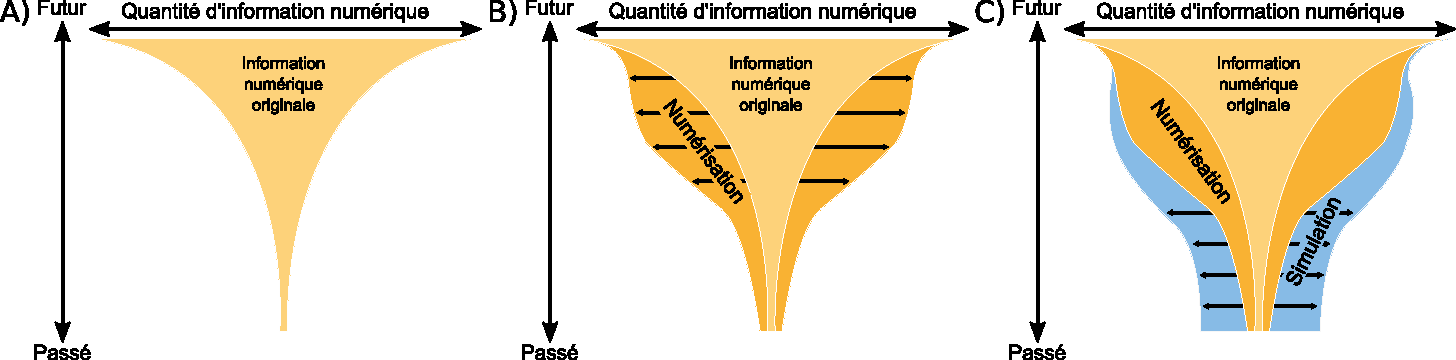
\includegraphics[width=\linewidth]{img/champignon_informationnel_kaplan.pdf}
	\caption{Le \og champignon informationnel\fg{}, d'après \textcite{kaplan_lancement_2013}.}
	\label{fig:champignon-kaplan}
\end{figure}

L'exercice de la modélisation demande pourtant une quantité substantielle de données, et surtout que ces données soient homogènes en termes de couverture spatio-temporelle et en termes de certitude face au risque que des \og effets de source\fg{} ne biaisent les résultats.
Afin d'augmenter la couverture spatio-temporelle, on a recours à des sources variées -- matérielles, écrites, voire biologiques -- par nature hétérogènes.

Les éléments empiriques ne peuvent dès lors reposer que sur une connaissance large et diversifiée des périodes et régions étudiées.
Cette connaissance, que l'on peut qualifier d'experte, est l'apanage des \og thématiciens\fg{} du projet.
Le modélisateur, qui ne peut acquérir l'ensemble des connaissances expertes des thématiciens, doit accepter de leur faire entièrement confiance quant aux éléments empiriques mobilisés dans le modèle et par l'intermédiaire desquels les modèles seront ensuite évalués.

Cela mène à une double implication en matière de légitimité.
Pour le modélisateur, cela implique qu'il sera toujours nécessaire de s'en remettre à la connaissance experte d'une personne (ou d'un groupe), sans possibilité d'ailleurs d'enrichir ces connaissances de son côté :
	mobiliser une référence scientifique dans une thématique de recherche inconnue ou distante, c'est risquer de citer des travaux non reconnus par la communauté, dépassés, ou encore anecdotiques.
Dans cette thèse, les tentations de référencer certains éléments empiriques en menant des recherches bibliographiques ont été nombreuses, mais sans vision d'ensemble de l'historiographie de ces sujets, cela n'ajouterait en fait aucun gage de scientificité.

Pour le thématicien, cela implique d'être en permanence \og malmené\fg{} par un modélisateur en recherche de connaissances plus précises et exhaustives.
Pierre \textsc{Garmy} le résume ainsi à propos de son expérience en tant que thématicien dans le projet TransMonDyn :
\begin{quotation}
\noindent \og La collaboration interdisciplinaire entre thématiciens et modélisateurs suppose le dépassement de deux contradictions : exhaustivité tendancielle \textit{vs} parcimonie recherchée d'une part et complexité \textit{vs} schématisation ou stylisation d'autre part.

\noindent Il existe un véritable paradoxe entre l'incomplétude de fait des données -- que les spécialistes disciplinaires cherchent à combler progressivement par l'enrichissement continu des corpus au moyen de recherches appropriées, rentabilisées par la définition de problématiques préalables aussi pointues que possible -- et l'attente des interlocuteurs modélisateurs qui veulent tout savoir et se bercent souvent d'illusions sur l'état de l'art réel dans chaque champ de connaissances. \fg{} \\
\mbox{}~ \textsc{Garmy} P., \og Annexe 1 - Retour sur expérience d'un “thématicien” \fg{}, in \textcite[476]{ouriachi_lelaboration_2017}  	  
\end{quotation}

\subsection{Un contexte fortement interdisciplinaire}

L'interdisciplinarité est le dernier élément marquant du contexte dans lequel ce travail de thèse a été initié et mené jusqu'à son terme.
Celle-ci est au cœur d'un projet tel que TransMonDyn, où collaboraient des géographes, archéologues et historiens, informaticiens et géomaticiens, épistémologues, linguistes, mathématiciens\ldots{}
Une expérience précédente, Archaeomedes \autocite{durand1998archaeomedes}, avait déjà posé les bases d'une certaine interdisciplinarité entre géographes et archéologues\footnote{
	On se réfère ici aux chercheurs en géographie humaine et, ou urbaine.
	En géomorphologie, géophysique et géographie environnementale, les collaborations entre géographes et archéologues, sur des questions techniques notamment, sont plus fréquentes et anciennes.
}, et plusieurs de ses membres historiques se sont donc retrouvés dans TransMonDyn.
Ce \og noyau dur\fg{} a constitué le pôle auxquels se sont agrégés d'autres chercheurs des disciplines mentionnées, et y compris en archéologie, des chercheurs qui avaient exprimé un désaccord quant aux approches très empreintes de systémique d'Archaeomedes \autocite[voir][par exemple]{ferdiere_modelisation_2000}.


Dans le projet TransMonDyn, on a souvent distingué les rôles des participants selon qu'ils étaient \og thématiciens\fg{}, porteurs de connaissance experte vis-à-vis des processus étudiés, ou \og modélisateurs\fg{}, porteurs d'une connaissance experte vis-à-vis de la manière de modéliser ces processus.
Au sein même de ces catégories, l'interdisciplinarité était fortement présente et a orienté les approches mises en place dans le projet.
%Au regard des enjeux du projet TransMonDyn, l'interdisciplinarité qui le caractérise s'exprime et contraint son ambition au moins de deux manières, que l'on pourrait rapporter aux domaines thématiques et méthodologiques.

\paragraph{Interdisciplinarité et thématique.}

En premier lieu, une forte interdisciplinarité entraîne nécessairement des points de vue disciplinaires différents sur des thématiques communes.
Il me semble que ces points de vue sont fortement liés aux sources manipulées.
Les données statistiques et issues d'enquêtes contemporaines de la géographie urbaine, les textes et la littérature grise historiques ou les traces et matériaux archéologiques, c'est-à-dire l'ensemble des éléments sur lesquels les disciplines se constituent, influencent fortement la manière de considérer un thème commun, comme celui de l'étude d'un système de villes par exemple.
Les géographes en analysent les interactions et populations au moyen de données de recensement ou d'analyses des comportements des acteurs territoriaux.
Les historiens se réfèrent aux sources historiques, le plus souvent issues des élites ou structures dominantes, qui communiquent sans doute des informations précises sur les liens politiques ou religieux entre les villes.
Les archéologues cherchent dans les traces matérielles des points communs en termes de nature de construction, de répartitions spatiales à l'échelle des lieux de fouilles afin d'identifier par exemple l'existence d'échanges entre les agglomérations.
Ces descriptifs, certes caricaturaux, montrent bien que pour une thématique commune, la disponibilité et la couverture spatio-temporelle des sources privilégiées par telle ou telle discipline orientent nécessairement l'approche.

Ces sources et perspectives différentes orientent aussi fortement les ontologies et lexiques utilisés.
On a donné l'exemple des villes, mais chaque discipline use de son propre jargon et se dote de concepts spécifiques pour le définir.
Un des défis de l'interdisciplinarité, du point de vue des thématiques, est alors de parvenir à tout expliciter, en usant d'un formalisme commun (définitions, ontologies\ldots), de manière à ne pas laisser de place à l'implicite disciplinaire.

Une approche variée, en termes de recherche d'explication des processus observés, découle nécessairement de ces différences de vocabulaire et de sources considérées.
Dans cette thèse, on a essayé de concilier les explications en intégrant l'ensemble des éléments constitutifs du système modélisé qui semblaient, pour l'un ou l'autre des thématiciens, pouvoir apporter une part d'explication.
Il fallait ainsi concilier la vision d'une géographe modélisatrice qui cherchait à expliquer la polarisation aux moyens d'attractions différenciées, la vision d'une archéologue pour qui les effets de lignages seigneuriaux et la territorialisation due aux paroisses permettaient de comprendre cette même polarisation et fixation, ou encore un historien pour qui les communautés rurales/agraires/paysannes émergentes étaient un facteur indispensable de la fixation de l'habitat rural.

Ce dernier point est aussi l'occasion d'estomper la différenciation, forte dans TransMonDyn, entre \og thématiciens\fg{} et \og modélisateurs\fg{}.
À mon sens, l'un des accomplissements de ce projet est aussi d'avoir montré que la frontière entre ces \og rôles\fg{} est fine, et extrêmement dépendante d'un positionnement particulier dans le cadre d'un projet particulier.
Au-delà du poncif qui reviendrait à dire que chacun est tour à tour modélisateur ou thématicien selon son interlocuteur, il me semble ainsi pouvoir retirer de l'expérience TransMonDyn que pour modéliser en interdisciplinarité, chacun doit en même temps adopter ces deux postures, devenant un \og modélicien\fg{} selon les termes d'Arnaud \textsc{Banos} :
\begin{quotation}
	\noindent \og Sous le néologisme “Modélicien”, je désignais un type d'interaction très différent, qui avait amené Robin Cura et Cécile Tannier, tous deux géographes et modélisateurs, à s'investir avec une telle intensité et une telle profondeur dans la problématique historique de leur groupe de travail qu'ils en étaient progressivement venus à s'exprimer comme s'ils avaient été eux-mêmes longuement formés à cette discipline (cf. [\cite{cura_transition_2017}]).
	L'évolution était tellement flagrante et systématiquement soulignée par les collègues historiens eux-mêmes que j'en suis même venu à émettre la possibilité d'un syndrome de TransMonDyn (en référence bien sûr au syndrome de Stockholm), défini de la manière suivante :
	“phénomène psychologique selon lequel des modélisateurs partageant longtemps la vie des thématiciens développent une empathie, voire une sympathie, ou une contagion émotionnelle avec ces derniers, devenant ainsi des modéliciens”.
	\fg{} \\
	\mbox{}~ \textsc{Banos} A., \og Annexe 3 - Petite typologie “empirique” des modélisateurs \fg{}, in \textcite[484]{ouriachi_lelaboration_2017}
\end{quotation}
Je crois que c'est là l'une des conditions permettant à un projet de passer de la pluridisciplinarité, \og juxtaposition disciplinaire\fg{} \autocite[14]{gravier_deux_2018}, à une interdisciplinarité définie comme une \og coopération de plusieurs disciplines autour de projets communs\fg{} (\cite[14]{gravier_deux_2018}, citant \textcite{AERES2014} p. 19).

\paragraph{Interdisciplinarité et méthodologie.}\label{par:interdisciplinarite-methodo}

Au-delà des difficultés que l'interdisciplinarité implique sur le plan thématique, on peut aussi en constater des retentissements en termes méthodologiques, très visibles dans le projet TransMonDyn.
La présence de géographes-modélisateurs, de géomaticiens, d'informaticiens, de mathématiciens ou encore de philosophes dans un projet génère nécessairement des approches diversifiées en matière de modélisation.
Le mathématicien favorisera en effet des formalismes mathématiques tels que les systèmes dynamiques ou la théorie des jeux, les philosophes préfèreront une modélisation ontologique des processus à l'œuvre, le géographe préfèrera une entrée spatiale, potentiellement statistique par exemple autour de modèles gravitaires, et l'informaticien usera de ses habitudes en modélisation à base d'agents, proches de la programmation à base d'objets communicants.

Le panorama des approches de modélisation mobilisées dans les transitions de TransMonDyn illustre cette diversité de pratiques :
	on y retrouve beaucoup de modèles à base d'agents, mais aussi des modèles basés sur la théorie des jeux, ou encore un modèle conceptuel basé sur une ontologie dynamique \autocite{favory_transition_2017}.
En considérant l'historique des approches de modélisation du projet, on pourrait de plus y ajouter des modèles graphiques, sagittaux ou chorématiques.
Ces approches ont en commun une vision systémique des processus, mais les modalités de leurs mises en place s'effectuent selon des langages (informatiques ou formels) et des paradigmes (mathématiques, statistiques ou informatiques) très différents.

Au sein même des modèles implémentés au travers de systèmes multi-agents, l'hétérogénéité est forte : entre un modèle KISS\footnote{
	Caractérisés ainsi par \textcite[110]{amblard_evaluation_2006} : 
	\og Un premier courant, qui est une application directe du rasoir d'Occam, aussi appelé  ``principe de parcimonie'', le mouvement KISS (Keep It Simple, Stupid !) recommande de construire des modèles qui soient analysables par la suite, suffisamment simples pour être disséqués par un humain qui observe les simulations attentivement \textelp{}.
	Le positionnement de ce courant peut se résumer ainsi : rien ne sert de concevoir des modèles dont on ne pourrait étudier sérieusement les propriétés et oublier ainsi la validation interne, définie comme l'existence des bonnes propriétés du modèle dans le cadre formel de ce dernier
	\fg{}.
}, un modèle descriptif, ou encore un modèle comportemental individu-centré, les paradigmes mobilisés sont entièrement différents et surtout ont des implications diamétralement opposées en matière de conception et d'évaluation.
L'interdisciplinarité, de manière générale, requiert une forte explicitation des concepts et méthodes employés.
Dans le cadre de projet collectifs de modélisation, c'est vrai pour l'aspect thématique -- chacun doit comprendre ce qui est modélisé afin de ne pas en mésinterpréter les résultats -- aussi bien que pour l'aspect méthodologique -- chacun doit comprendre la manière dont les objets sont modélisés pour les mêmes raisons.
L'interdisciplinarité, sur le plan méthodologique, demande donc aussi une forte explicitation afin d'assurer la compréhension partagée des méthodes mises en places, des biais qu'elles impliquent, et des limites qu'elles comportent.

%
%C'est vrai aussi bien pour l'aspect thé
%Du point de vue méthodologique, l'interdisciplinarité dans la conception de modèles requiert, comme pour les aspects thématiques, une forte explicitation des concepts et méthodes employés afin que l'ensemble des parties prenantes soient d'une part satisfaits des modèles produits, et d'autre part en capacité de comprendre les hypothèses et biais intrinsèques qui découlent du choix du type de modélisation.

\bigskip
\paragraph[Conclusion intermédiaire]{}

Le contexte dans lequel cette thèse a été imaginée et initiée, retracé dans cette partie, permet de mieux comprendre les enjeux -- méthodologiques et thématiques -- de ce travail.
Les membres du groupe de travail de la \og transition 8\fg{} de TransMonDyn ont continué à œuvrer ensemble, même après les fins officielles (2014) et effectives (2017, à la parution de l'ouvrage collectif \og Peupler la Terre\fg{} dirigé par \textcite{sanders2018peupler}) de ce projet de recherche interdisciplinaire.
Le modèle SimFeodal, et cette thèse plus largement en constituent l'un des aboutissements.

Ma thèse, en tant que telle, n'a pourtant pas été réalisée dans le cadre officiel de l'ANR TransMonDyn.
Le présent travail de thèse a ainsi bénéficié d'un financement du LabEx DynamiTe\footnote{
	Laboratoire d'Excellence \og Dynamiques Territoriales et Spatiales\fg{}, ANR-11-LABX-0046, dans le cadre du programme \og Investissements d'Avenir\fg{}.
}, proposé par le groupe de travail \og Systèmes de Peuplement sur le temps long\fg{}\footnote{
	Co-dirigé par Patrice \textsc{Brun}, Marie-Vic \textsc{Ozouf-Marignier} et Lena \textsc{Sanders}.
}, dont l'objectif initial était de \og croiser les connaissances et savoir-faire de géographes, historiens, archéologues et mathématiciens pour décrire, conceptualiser et modéliser les dynamiques du peuplement sur le temps long dans leurs expressions spatiales et leurs rythmes temporels\fg{}\footnote{
	Descriptif du groupe de travail : \href{http://labex-dynamite.com/fr/recherches/groupes-travail/les-systemes-de-peuplement-sur-le-temps-long/}{http://labex-dynamite.com/fr/recherches/groupes-travail/les-systemes-de-peuplement-sur-le-temps-long/}
}.
Au regard de ces objectifs, on comprendra aisément les similarités avec TransMonDyn, que ce soit en termes d'interdisciplinarité ou de démarche.

Dans les faits, ce groupe de travail \og temps long\fg{}, dans lequel je me suis inscrit tout au long de mon travail de thèse, a surtout œuvré à la résolution d'une des difficultés de l'interdisciplinarité décrite plus haut : la mise en place d'un vocabulaire commun et explicite sur les concepts et notions liés à la description et à la modélisation des systèmes de peuplement sur le temps long.
La réalisation d'un \og lexique spatio-temporel illustré\fg{}\footnote{
	C'était le nom provisoire, modifié par la suite, de ce projet.
} qui résulte de ce projet, intitulé \og Les concepts-clés des systèmes de peuplement sur le temps long \fg{} \autocite{sanders_les_2020}, a nourri l'ensemble de cette thèse, en contribuant largement à mettre au clair les concepts employés.
À ce titre, le groupe de travail du LabEx a aussi constitué un contexte fort, en mettant en place des discussions interdisciplinaires, autour des mêmes disciplines mais avec des communautés de chercheurs et d'approches distinctes de celles de TransMonDyn.

\let\orisectionmark\sectionmark
\renewcommand\sectionmark[1]{}%
\section[Conditions et modalités de la modélisation collective et interdisciplinaire]{Du projet de thèse à une question de recherche : les conditions et modalités de la modélisation collective et interdisciplinaire \label{sec:evolution}}
\orisectionmark{Conditions et modalités de la modélisation collective et interdisciplinaire}
\let\sectionmark\orisectionmark

Entre mon projet de recherche initial, proposé au LabEx DynamiTe, et le présent rendu, le sujet, les questionnements et surtout les approches mises en places pour y répondre ont fortement évolué.
Les grands axes du positionnement sont eux restés constants, de même que la thématique d'ensemble.
Le titre initial de ce projet montre qu'il s'agit plus d'un changement de point de vue sur les approches à mobiliser que sur le thème en lui-même.
Ce projet s'intitulait en effet originellement \og Exploration et analyse de données spatio-temporelles : application à la modélisation des transformations des systèmes de peuplement sur le temps long\fg{}.
On notera que les principales idées sont communes au titre actuel (\og Accompagner la modélisation des systèmes de peuplement par l'exploration interactive de données spatio-temporelles \fg{}\footnote{
	\hl{A corriger avec titre définitif.}
}), mais que l'ordre en a été bouleversé, que la logique d'accompagnement a été mise en avant (même si elle était mentionnée dans le projet de recherche, cf. \textit{infra}) et que certaines composantes ont été spécifiées.

Le programme de recherche initial était orienté autour de trois tâches :

\begin{compactenum}\vspace*{-.5em}
	\item \og Mise en place d'une démarche d'accompagnement des thématiciens dans la modélisation\fg{} ;
	\item \og développement d'une plateforme d'exploration de données spatio-temporelles : application à des transitions dans le système de peuplement\fg{} ;
	\item \og analyse des transitions du système de peuplement modélisées\fg{}.
\end{compactenum}\vspace*{-.5em}

Ces grandes dimensions d'analyses sont toujours présentes, largement ré-organisées et hiérarchisées différemment.
Il s'agit ici de revenir sur les obstacles et solutions rencontrées durant le travail de thèse, qui ont conduit à reformuler et ré-agencer ces trois composantes initiales.
%Sans faire un retour complet et exhaustif sur les évolutions de ma recherche, il me semble utile ici de revenir sur ces éléments\footnote{
%	Les titres des sous-parties reprennent les trois tâches du projet initial, mais ont été renommées pour une meilleure correspondance au contenu final du projet.
%}, les obstacles qu'ils ont rencontrés et les solutions choisies pour les résoudre.
%Cela permettra de mieux cerner le positionnement de ce travail dans le champ de la modélisation en géographie.



\subsection[Position du modélisateur : du guide au con-constructeur]{Position du modélisateur : du guide au con-constructeur}

L'ambition d'origine était d'accompagner la modélisation des transitions en \og [extrayant] les connaissances des thématiciens et [en les décryptant] afin d'en tirer des processus de causalité, de dépendance et d'inter-relations\fg{}.
Il me semble maintenant que le terme de \og guider\fg{} la modélisation aurait plus fidèlement représenté l'approche qui était initialement prévue.
Il s'agissait ainsi plutôt d'orienter et de diriger les thématiciens vers la conception de modèles plutôt que de le faire avec eux, en m'adaptant aussi à leur point de vue.


\paragraph{Guider la modélisation de cas d'études suivant une approche harmonisée.}

Dans les faits, en matière d'accompagnement, mon projet de recherche initial visait à formaliser les discours experts des thématiciens en vue de leur modélisation.
Cette formalisation devait s'appuyer sur des méthodes graphiques à l'aide de \og briques de bases\fg{}, modèles schématiques d'un type de processus ou d'interaction.
Pour que cette approche soit généralisable à toutes les transitions identifiées dans TransMonDyn, il fallait alors que celles-ci atteignent une certaine homogénéité dans le degré de maturité de leur conceptualisation, et donc que l'ensemble des thématiciens acceptent ce type de modélisation généralisant.
Il s'agissait donc de modéliser, à partir des connaissances expertes, et éventuellement des données empiriques disponibles, voire à partir de modèles déjà réalisés par les groupes de travail, chacune des transitions selon un paradigme commun et générique.

D'une part, on le constate à la lecture de l'ouvrage collectif issu du projet TransMonDyn, les modèles ont atteint des niveaux d'avancement très inégaux.
D'autre part, ils ont aussi été réalisés selon des paradigmes tout aussi variés dans leur démarche (plutôt KISS ou KIDS, différents niveaux d'agentification, etc., cf. \nameref{par:interdisciplinarite-methodo}, p. \pageref{par:interdisciplinarite-methodo}).
Un type générique de modélisation, même sans aller jusqu'à l'implémentation effective, n'était donc pas applicable à l'ensemble des transitions.
Une solution aurait été de sélectionner un sous-ensemble des transitions, homogène en terme d'approche et de progression vis-à-vis de l'implémentation.
Là encore, chaque modélisateur ayant une approche propre (voir plus haut), une telle homogénéité était pourtant difficilement identifiable.
%Il était alors nécessaire d'en sélectionner un sous-ensemble homogène, ce qui est difficilement possible quand les modélisateurs impliqués dans la modélisation présentent une diversité d'approches.

En allant plus loin, on peut noter que même dans le cas du projet TransMonDyn où un même modélisateur a collaboré à plusieurs transitions, il a choisi de développer des types de modèles très différents.
Alain \textsc{Franc}, un mathématicien qui a participé aux transitions 9 \autocite{ouriachi_transition_2017} et 12 \autocite{bretagnolle_transition_2017}, voir \cref{tab:transitions-tmd}, a ainsi choisi d'utiliser la théorie des jeux dans le premier cas, et de réaliser un modèle descriptif statique dans le second.
Cet exemple met en exergue l'obstacle qui me paraît désormais majeur dans la conception de modèles différents selon un formalisme et un paradigme harmonisé : le type de modèle est un choix collectif des membres impliqués, mais il n'est pas pour autant réalisé de manière entièrement indépendante.
Le questionnement initial, les données disponibles ou encore le parcours personnel des membres impliqués jouent ainsi un rôle considérable dans les choix de modélisation.

En premier lieu, le parcours méthodologique et scientifique de chacun des participants joue un large rôle, chaque modélisateur ayant naturellement tendance à approcher un problème avec les outils qu'il a l'habitude d'utiliser.
Un statisticien habitué aux systèmes dynamiques à base d'équations différentielles aura du mal à concevoir un modèle conceptuel en termes d'agents et de mécanismes, et un adepte des modèles à base d'agents très parcimonieux sera sans doute frustré par un choix collectif de modèle descriptif.
%Cela explique qu'Alain \textsc{Franc} n'ait pas mené de modélisation à base d'agents dans ces exemples.

En second lieu, il me semble que la combinaison du questionnement initial et la nature des données disponibles conditionne aussi très largement le choix du type de modélisation.
Selon que le questionnement repose sur l'observation de dynamiques individuelles ou au contraire agrégées, on se tournera ainsi soit vers des méthodes où l'individu peut être suivi (modèles agents, théorie des jeux, etc.), soit vers des méthodes plus agrégeantes (systèmes dynamiques par exemple).
Selon que le questionnement porte sur le déroulement des \og transitions\fg{} ou au contraire sur la caractérisation des \og régimes\fg{}, on choisira aussi différentes méthodes.
Au niveau des données empiriques, plus celles-ci sont nombreuses, plus le type de modélisation pourra être \og \textit{data-driven}\fg, produisant peut-être des modèles plus parcimonieux donnant une forte importance à la validation.
Au contraire, en présence de peu de données empiriques mais de nombreuses connaissances expertes, des modèles \og theory-driven\fg{} seront sans doute privilégiés, évalués et mobilisés de manière plus qualitative.
Dans l'exemple du projet TransMonDyn, le choix de la modélisation agent, basée sur des connaissances expertes et non sur les données, a été un choix collectif décidé dès le début du projet.
Ce n'est donc pas la disponibilité des données qui a influencé le type de modélisation, sauf peut-être pour la modélisation de l'une des transitions \autocite{bretagnolle_transition_2017}, où les nombreuses données disponibles et leur format ont encouragé à la création d'un modèle statistique descriptif.


\paragraph{De la prescription à l'accompagnement.}

Au-delà de la question de la faisabilité effective d'un tel projet d'accompagnement global à la modélisation d'un ensemble de transitions, rendue difficile dans le contexte très interdisciplinaire et multi-approches de TransMonDyn, la réalisation de cet \og accompagnement à la modélisation\fg{} posait question en matière de méthode d'accompagnement.
Dans un tel contexte, la proposition d'un cadre conceptuel commun et générique de modélisation était-elle la manière la plus adaptée de réellement \og accompagner\fg{} la modélisation ?
Dans un parcours, un accompagnateur peut ainsi être devant, au même niveau, ou derrière ceux qu'ils accompagnent.
La position que j'avais initialement prévue me plaçait \og devant\fg{}, c'est-à-dire en guide chargé d'orienter la marche des suivants en proposant un seul itinéraire, c'est-à-dire une approche commune et unique de modélisation.
Cela n'a pas été possible pour une raison chronologique triviale -- le projet TransMonDyn avait commencé avant le début effectif de cette thèse --, mais aussi vis-à-vis des discussions collectives relatives à la position des modélisateurs, unanimement choisie comme une position d'accompagnement \og au même niveau\fg{} pour reprendre la métaphore précédente.
%Surtout, cette posture de modélisateur \og imposant\fg{} ses propres outils et approches de modélisation ne pouvait s'inscrire dans un projet à volonté réellement interdisciplinaire tel que TransMonDyn.
%D'une part, parce que \og le modélisateur n'est pas omni-compétent\fg{} \autocite[77]{banos_pour_2013}, et d'autre part parce que le \og le modélisateur doit cesser de proposer des solutions uniques et optimales à des problèmes complexes\fg{} \autocite[79]{banos_pour_2013}.
Cela interroge le positionnement du modélisateur vis-à-vis des thématiciens \og avec\fg{} lesquels il cherche à concevoir un modèle, et qui voulait, dans TransMonDyn, être celui d'un \og accompagnateur\fg{} et co-acteur plus que celle d'un prescripteur ou d'un assistant technique.


J'ai très vite réalisé que la proposition d'un cadre commun de modélisation ne pouvait fonctionner au regard des spécificités de chacune des approches mises en places pour décrire les transitions.
Pour que chacun investisse son temps et son énergie dans une expérience de modélisation, qui peut se montrer frustrante pour les thématiciens \autocite[470]{ouriachi_lelaboration_2017}, il faut avant tout veiller à répondre aux attentes de ces derniers vis-à-vis de l'usage du modèle.
En d'autres termes, pour que des chercheurs consacrent du temps à un travail, encore faut-il que celui-ci leur apporte quelque chose.
L'identification de qui \og profite\fg{} d'un modèle\footnote{
\og who benefits in what manner from the simulation\fg{} selon les mots de \textcite[260]{lake_trends_2014}
} est claire dans le cadre commun de la \og modélisation d'accompagnement\fg{} \autocite[voir][par exemple]{etienne_modelisation_2015}, où l'on cherche à sensibiliser une population aux dangers et risques qu'elle encoure.
Dans le cadre d'un projet de recherche où les objectifs des modèles sont plus théoriques, où les attentes vis-à-vis des modèles sont plus diversifiées, voire où des réticences vis-à-vis de la modélisation peuvent être présentes, il me semble qu'une conception collective du modèle et de l'approche de modélisation est la seule susceptible de rassembler les énergies nécessaires.

Dès lors, la modélisation ne pouvait se faire qu'en gardant à l'esprit, constamment et tout au long, les attentes et envies de chacune des parties prenantes.
Cela n'est pas possible dans une approche prescriptrice de \og modélisateur éclairé\fg{} \autocite[484]{ouriachi_lelaboration_2017}.
Un consensus permanent sur la manière de procéder est ainsi nécessaire, sous risque de voir l'expérience échouer avant son terme.
Pour que le projet de modélisation interdisciplinaire aboutisse, le modélisateur ne peut être un simple \og implémenteur\fg{}, qui ne participerait qu'à la dernière phase -- l'implémentation informatique du modèle conceptuel.
Comme le relate Arnaud \textsc{Banos} :
\begin{quotation}
	\noindent \og
	Le travail en interdisciplinarité suppose une alchimie particulière, dont l'existence n'est jamais acquise et qui doit être entretenue, nourrie en permanence.
	Dans cette quête incessante et toujours renouvelée, les interactions entre modélisateurs et non modélisateurs -- surtout si ces derniers s'inscrivent dans des disciplines relevant des sciences humaines et sociales -- prennent une saveur tout à fait singulière \textelp{}
	
	\noindent L'alchimie dont je parlais au tout début de mon propos suppose une certaine forme d'intimité.
	Et du temps.
	Une denrée de plus en plus rare dans nos métiers. \fg{} \\
	\mbox{}~ \textsc{Banos} A., \og Annexe 3 - Petite typologie “empirique” des modélisateurs \fg{}, in \textcite[483,485]{ouriachi_lelaboration_2017}
\end{quotation}
Ne disposant pas du temps nécessaire, ni pour créer cette intimité avec chaque groupe de travail, ni pour mener la modélisation de plusieurs transitions, j'ai considéré que mieux valait se concentrer sur la modélisation d'une unique transition.
C'est ainsi qu'il était possible d'y investir le temps suffisant, plutôt que de chercher à multiplier les expériences de modélisation de plusieurs transitions, ce qui aurait pu être frustrant pour les thématiciens et autres modélisateurs impliqués.


\subsection{Explorer plutôt que confronter des données empiriques et simulées}

La deuxième tâche du projet initial de thèse était de construire une plate-forme interactive dédiée conjointement à l'exploration des données empiriques sur lesquelles sont fondées les modèles, à l'exploration des données simulées produites par ces modèles, et enfin à la confrontation de ces données empiriques et simulées.
La structure des données disponibles a entrainé une reformulation de cette ambition.

\paragraph{D'une modélisation descriptive à une modélisation dynamique.}

L'idée sous-jacente était de compléter les connaissances expertes autant que possible en mobilisant les données empiriques existantes afin de faciliter/accélérer/détailler les faits stylisés identifiés lors de la conception des modèles conceptuels.
Je savais que les archéologues, en particulier, du projet TransMonDyn s'appuyaient sur de vastes corpus de données correspondant à l'enregistrement et à la formalisation informatique de matériaux issus de fouille.
Les transitions portées par des géographes, elles-aussi, pouvaient compter sur des données exhaustives et complètes sur le territoire et les périodes étudiées.
J'envisageais donc de créer un outil permettant à chacun, thématiciens compris, d'explorer les données compilées pour chaque transition, et ainsi de contribuer à y trouver des corrélations, des récurrences spatio-temporelles ou autres motifs dans les données qui auraient pu enrichir et faciliter la conception des modèles.

Dans les faits, et c'est aussi une limite qui n'est visible qu'une fois l'exercice entamé, l'utilisation des données archéologiques est bien plus complexe que je ne pouvais le prévoir en tant que géographe habitué aux sources de données contemporaines, institutionnelles et souvent exhaustives.
De nombreuses \og données\fg{} existent, mais elles ne sont par forcément harmonisées ou homogènes, et surtout, elles sont très lacunaires sur les dimensions temporelles (des périodes entières ne sont pas couvertes) et spatiales (les données ne couvrent que rarement l'ensemble du territoire étudié).
À une exception près, les modèles finalement issus de TransMonDyn sont d'ailleurs tous \og \textit{theory-driven}\fg{} plutôt que \og \textit{data-driven}\fg{}\footnote{
	Pour une bonne comparaison de ces approches, voir \textcite[120--122]{mathian_objets_2014}.
} :
	ils reposent sur des connaissances expertes et des hypothèses thématiques plutôt que sur une information quantifiée qui serait directement injectée dans les modèles.
Dans la plupart des cas\footnote{
	À l'exception de la transition 9 (cf. \cref{tab:transitions-tmd}) où les auteurs \autocite{bretagnolle_transition_2017} ont justement mené un travail de modélisation \og statique\fg{} à partir des données disponibles, en modélisant les états successifs des potentialités d'échanges inter-urbains plutôt que de modéliser les causes de leur émergence. 
}, les données en tant que telles ont été mobilisées comme des moyens d'évaluer les modèles plutôt que comme des bases de construction.
L'usage des données empiriques, dans ma thèse, s'inscrit pleinement dans cette approche empruntée collectivement par les participants du projet TransMonDyn.
%Il aurait été vain de vouloir explorer ces données, hétérogènes au sein même des transitions, pour espérer en tirer une quelconque connaissance qui aurait complétée l'expertise thématique de chercheurs ayant étudié des thématiques localisées et datées pendant des dizaines d'années.

\paragraph{Exploration de modèles et confrontations de données.}

Pour \og explorer les modèles\fg{}, c'est-à-dire analyser l'étendue des dynamiques simulées et des sorties auxquels ils pouvaient aboutir, et mener ainsi une validation de ces modèles, je comptais mobiliser des méthodes d'exploration automatisée de modèles.
Le projet ERC GeoDiverCity\footnote{
	ERC Advanced Grant 269826 GeoDiverCity, dirigé par Denise \textsc{Pumain} - \\ \href{http://geodivercity.parisgeo.cnrs.fr/blog/}{http://geodivercity.parisgeo.cnrs.fr}
}, auquel je contribuais par ailleurs, comportait en effet un axe de recherche sur le développement de telles méthodes.
Dans ce cadre, des outils et algorithmes d'exploration automatisée de modèles avait déjà été développés lors de la rédaction de mon projet initial de thèse.
Plusieurs thèses issues de ce projet ERC avaient ainsi privilégié ce type d'approches pour explorer les modèles \autocite{schmitt_modelisation_2014,cottineau_levolution_2014,rey-coyrehourcq_plateforme_2015}.

Fondamentalement, le présupposé de telles méthodes (\hl{cf chap7}) est que les modèles construits soient aussi parcimonieux que possibles, dotés d'une quantité minime de paramètres et d'indicateurs de sortie.
En automatisant les analyses, il aurait été aisé de confronter ces sorties aux données empiriques disponibles, la simulation informatique ayant l'énorme avantage de laisser au modélisateur choisir le format, le type et la quantité des données générées.

Le contexte effectif de co-construction du modèle a pourtant invalidé, ou au moins freiné, ce type d'approche.
Ces méthodes d'exploration automatiques sont en effet pensées comme permettant l'exploration de modèles plutôt KISS.
Pour mener une exploration complète, il faut minimiser le nombre de paramètres en entrées et le nombre d'indicateurs en sortie.
Dans le cas inverse, l'\og explosion combinatoire\fg{} qui résulte de leurs combinaisons empêche de mener une exploration complète.

La réalisation de modèles KISS demande cependant aux thématiciens de faire preuve d'une forte abstraction quant aux processus et entités modélisés.
Dans un contexte de premières expérience de modélisation pour une large part des thématiciens du projet TransMonDyn, cela rendait difficile l'adoption de ce type de modélisation qui demande \og un apprentissage, une familiarisation progressive avec un mode de pensée qui n'est pas génétiquement le sien\fg{} (\textsc{Garmy} in \cite[477]{ouriachi_lelaboration_2017}).
Pour des néo-modélisateurs, le choix de modèles KIDS est alors plus aisé, et le travail de \og parcimonisation\fg{} qu'implique ce type de modèle dans un second temps aide justement à cette \og familiarisation progressive\fg{}.

Avec des modèles plutôt descriptifs, la tâche d'exploration est plus complexe, sans parler même d'une éventuelle validation.
Cette exploration des modèles, à partir des données issues de simulation, ne peut être que manuelle.
À ce titre, la plate-forme interactive de confrontation des données pouvait avantageusement être repensée pour servir à l'exploration des données simulées.
Au lieu de comparer des données empiriques et des données de simulation, elle servirait à explorer des données simulées, et à les confronter à d'autres données simulées afin de pouvoir comparer différents modèles ou versions de modèles par l'entremise de l'exploration interactive de données.

\subsection{D'un méta-modèle à un retour sur expérience de modélisation}

Le projet initial visait enfin à aller vers l'expression d'un modèle générique de transition dans les systèmes de peuplement -- un méta-modèle --, qui serait issu d'une analyse comparée des différents modèles.
La conception d'un tel méta-modèle ne pouvait se passer d'analyses poussées de plusieurs modèles de transitions, formalisés de la même manière et avec des approches homogènes.
En d'autres mots, sans avoir \og guidé\fg{} la modélisation de plusieurs cas d'études, ou sans intervenir complètement après l'achèvement du projet TransMonDyn, une fois que toutes les transitions auraient déjà été modélisées, il était invraisemblable d'aboutir à un tel résultat.

Cet objectif s'avérant peu réalisable au regard du contexte effectif de cette thèse, et au fur et à mesure du travail collectif de modélisation dans lequel je me suis trouvé impliqué, j'ai accordé une importance de plus en plus sensible à l'un des moyens de parvenir au méta-modèle qui avait été identifié dans le projet de thèse initial.
Il s'agissait de la \og la mise en place d'une démarche facilitant le dialogue et la compréhension interdisciplinaire\fg{}.
À force de ré-ajustements de ce travail de thèse, c'est en définitive dans cette direction que j'ai dirigé mon travail, en cherchant à concevoir des \og interfaces\fg{}, méthodologiques et techniques, à la modélisation.
Ces interfaces, détaillées par la suite (\cref{subsec:interfaces}), ambitionnent d'aider à la modélisation des transitions d'une manière qui soit satisfaisante pour chacun des acteurs impliqués, modélisateurs compris.
C'est cette démarche qui est précisée dans la partie suivante et que l'ensemble de la thèse cherche à définir sur la base d'un retour sur une expérience fructueuse de modélisation interdisciplinaire.
Elle permet de définir mon positionnement dans le champ de la modélisation géographique.


\let\orisectionmark\sectionmark
\renewcommand\sectionmark[1]{}%
\section{Visualiser et explorer pour co-construire un modèle : conception d'interfaces exploratoires}
\orisectionmark{Visualiser et explorer pour co-construire un modèle : conception d'interfaces exploratoires}
\let\sectionmark\orisectionmark

Les parties précédentes ont permis de définir et de préciser l'objet de recherche de ce travail de thèse, la modélisation de transitions dans le système de peuplement.

Le contexte dans lequel la thèse s'est déroulée (\cref{sec:contexte}), entre les projets TransMonDyn et le groupe de travail \og temps long\fg{} du LabEx DynamiTe, a amené ce thème et montré les enjeux de la modélisation des transitions comme objet de recherche interdisciplinaire, fait de l'étude de processus spatiaux complexes et de leur inscription dans le temps long.

Ma formation initiale et son extension en tant qu'ingénieur d'étude à l'UMR Géographie-cités (\cref{sec:formation}) ont orienté le choix des méthodes :
	mobiliser le cadre méthodologique des modèles à base d'agent, en donnant une forte place aux mécanismes géographiques et géométriques, et veiller à l'importance de la représentation graphique dans leur usage.

Le questionnement initial et son évolution (\cref{sec:evolution}) ont permis de recentrer le sujet d'ensemble de cette recherche.
Depuis la volonté initiale de créer un méta-modèle, il s'agissait désormais de documenter et promouvoir l'approche d'ensemble mise en place tout au long de ce travail collectif et interdisciplinaire.

Dans cette dernière partie, je souhaite préciser et justifier cette approche de modélisation interdisciplinaire qui est (1) résolument inscrite dans la co-construction et (2) s'appuie sur la mise en places d'interfaces disciplinaires (thématiques et méthodologiques) pour faciliter cette co-construction interdisciplinaire.
Cette approche est (3) délibérément exploratoire, aussi bien pour la conception du modèle que pour son analyse, tout en visant à (4) assurer une reproductibilité des moyens, méthodologiques et techniques, mis en œuvre.


\subsection{Favoriser une co-construction interdisciplinaire}

Quand on cherche à initier une démarche de modélisation collective, qui plus est en situation d'interdisciplinarité, les approches de \og modélisation d'accompagnement\fg{} (\og ComMod\fg{}, pour \textit{companion modelling}) paraissent incontournables dans le champ francophone de l'étude des systèmes complexes.
Il me semble dès lors important de positionner l'approche défendue dans cette thèse vis-à-vis de la modélisation d'accompagnement, et d'en identifier les points communs et de divergence.

\paragraph{Animer un projet interdisciplinaire.}

L'approche ComMod est définie par ses créateurs comme \og une démarche permettant de faciliter des processus collectifs de décision, en proposant un travail d'explicitation des points de vue et des critères subjectifs auxquels se réfèrent implicitement, voire inconsciemment, les différentes parties prenantes\fg{} \autocite[167]{commod_modelisation_2005}.
Les partisans de cette approche utilisent la modélisation de systèmes complexes comme un outil d'interface entre les différents acteurs d'une problématique souvent environnementale.
Cette modélisation est pensée comme véritablement collaborative, le modèle servant de support de discussion et de négociation entre des acteurs parfois opposés.
La démarche mobilisée, bien ancrée dans le paysage de la modélisation de systèmes complexes, se fonde autour de \og cinq étapes incontournables\fg{} \autocite[41-132]{etienne_modelisation_2015} :
\begin{compactenum}\vspace*{-0.5em}
	\item Identifier et formuler une question clé initiale partagée ;
	\item Co-construire une représentation partagée de la question (méthode \og ARDI\fg{}) ;
	\item Concevoir et animer un jeu de rôles ;
	\item Concevoir et développer un modèle informatique ;
	\item Suivre le développement et évaluer les effets de la démarche.
\end{compactenum}\vspace*{-0.5em}

Cette approche émane de chercheurs impliqués dans des opérations de \og recherche-action\fg{} \autocite[165]{commod_modelisation_2005}, et donne dès lors une importance prépondérante au travail de terrain \autocite[3.3]{barreteau_our_2003}, en particulier comme méthode d'évaluation des modèles produits.
Les modélisateurs y sont d'ailleurs présentés comme des \og animateurs\fg{}\footnote{
	Dans la méthode \og ARDI \fg{} (Acteurs, Ressources, Dynamiques et Interactions) \autocite{etienne_co-construction_2009} qui est au cœur de la démarche ComMod.
}, dont l'objectif est de pousser au dialogue les \og participants\fg{}, décideurs politiques, acteurs de la société civile ou encore population potentiellement à risque dans les programmes de sensibilisation.

Cette dichotomie entre \og animateurs\fg{} et \og participants\fg{} peut rappeler celle que l'on fait entre \og modélisateurs\fg{} et \og thématiciens\fg{}, mais elle y ajoute une hiérarchie en termes de maîtrise du processus de modélisation dans son ensemble.
Dans cette thèse, je défends une approche \og démocratique\fg{}, où le modélisateur n'a pas pour vocation de guider les thématiciens, mais bien de construire avec eux, de manière collective, c'est-à-dire de co-construire.

L'utilité d'un \og animateur\fg{}, qui peut être modélisateur comme dans la démarche ComMod mais aussi thématicien, est toutefois incontestable, notamment pour initier réellement le projet collectif et, de prime abord, réussir à concilier les intérêts thématiques et méthodologiques de chacun des membres impliqués -- animateur compris -- autour d'un objectif consensuel commun.
Dans le groupe de travail de la \og transition 8\fg{} de TransMonDyn, c'est Cécile \textsc{Tannier} qui a joué ce rôle d'animatrice, en mobilisant son expérience de modélisation pour amener les thématiciens à concevoir collectivement un premier modèle conceptuel de la transition, sous la forme d'une ontologie \autocite{tannier_ontologie_2014}.

\paragraph{Un projet collectif et intégrateur.}

Dans l'approche ComMod, l'implémentation informatique des modèles conceptualisés est une option, concurrente au développement d'un jeu de rôle, qui peut être mieux adaptée aux problématiques modélisées \autocite[96-97]{etienne_modelisation_2015}.
Le modèle de simulation joue donc le rôle de compagnon dans le processus de modélisation, mais n'est pas un objectif en soi.
Le développement du modèle de simulation demande ainsi des compétences informatiques particulières.
Celles-ci sont difficiles ou peu stimulantes à acquérir dans le cadre d'un projet caractérisé par le \og peu de temps disponible et l'hétérogénéité des savoir-faire informatiques des participants et la diversité de leurs attentes en la matière\fg{} \autocite[29]{etienne_modelisation_2015}.

D'après ma compréhension de la démarche ComMod, l'implémentation est alors le plus souvent réalisée par des modélisateurs externes au projet et le modèle permet de tester les hypothèses des participants ou de les faire évoluer.
Le modélisateur-informaticien est placé dans une position extérieure mais aussi surplombante.
D'où un risque que le modèle implémenté soit considéré comme \og l'implémentation\fg{} du modèle conceptuel plutôt que comme une de ses implémentations possibles, et constitue donc l'unique référentiel d'évaluation de la démarche.
Les participants sont ainsi inscrits dans une démarche clientéliste, plus proche de la pluridisciplinarité que de l'interdisciplinarité, que le texte suivant de \textsc{Tukey} me semble bien résumer, en remplaçant le \og statisticien\fg{} par l'\og{}informaticien modélisateur\fg{}.

\begin{quotation}
	\noindent \og Like every other methodology, statistical-and-quantitative methodology has fostered a separation of roles, here into “statistician” and “client”. Today theses roles are usually embodied in separate people. Tomorrow more persons will play both roles. But these roles will not melt together, and the need to consult another person will not altogether disappear [...]
	
	Too often the client (whether or not a social scientist) looks to the statistician as a man who applies the final stamp of approval -- perhaps by saying, “This result is significant”. Too often the statistician looks upon himself as a guardian of the proven truth -- sometimes feeling it appropriate to say “That difference is not significant at 5\%, \textit{and hence} you should act as if it were \textit{zero}”. The roles of “client seeking stamp of approval” and “statistician guarding the proven truth” are clearly rewarding to client and statistician respectively, as persons, though they are detrimental to progress and to the advance of science.\fg{} \\
	\mbox{}~ \hfill \cite[145]{jones_statistical_1986}
\end{quotation}

Pour la conception et l'implémentation de SimFeodal, nous avons cherché à suivre une approche plus intégratrice, en séparant moins nettement les rôles de thématicien, de modélisateur, voire d'\og{}implémenteur\fg{}.
Si chacun de ces rôles correspond à des compétences particulières peu accessibles aux autres, l'idée était tout de même d'échanger au maximum sur chacun des aspects du modèle de manière à les rendres plus compréhensibles pour tous.
Par exemple, on souhaitait que les raisons thématiques d'un choix de valeur de paramètre soient explicitées, justifiées et partagées par les thématiciens auprès les modélisateurs.
À l'inverse, les modélisateurs devaient expliciter les partis-pris, biais ou encore alternatives des choix d'implémentation effectués, par exemple en détaillant le point de vue adopté dans l'implémentation d'un mécanisme concernant les actions d'un type d'agent (cf. \hl{encadré chap2}).

Sans chercher à ce que chacun des chercheurs impliqués dans la construction de SimFeodal ne devienne omnicompétent, notre approche visait toutefois, dans la mesure du possible, à ce que chacun soit en mesure de comprendre et donc de défendre, au moins dans les grandes lignes, les choix de modélisation et d'implémentation qui seraient réalisés.

\paragraph{Une position de \og modélisateur-géographe\fg{}.}

Dans cette approche de co-construction, on essaie de faire en sorte que chacun partage un socle de connaissances commun de manière à pouvoir comprendre les implications des différentes décisions, conceptuelles, méthodologiques ou techniques.
Thématiciens et modélisateurs doivent donc tendre vers un objectif idéal de transdisciplinarité, où les points de vue disciplinaires s'effacent et se confondent \autocite[14]{gravier_deux_2018}.
Pour reprendre l'expression de \textsc{Banos} (in \textcite[]{ouriachi_lelaboration_2017}), dans un processus de co-construction absolu, chacun devrait devenir \og modélicien\fg{}.

En pratique, chacun a toutefois ses compétences et connaissances spécifiques et ne cherche pas à acquérir entièrement celles des autres.
La position de co-construction effective est donc bien celle de l'interdisciplinarité, complémentaire autour de sujets communs, et non celle de la transdisciplinarité.

Il me semble en effet que ces points de vue disciplinaires sont d'une part difficilement \og effaçables\fg{} dans des rôles donnés, et d'autre part extrêmement enrichissants dans un projet de co-construction.
Ma position, en tant que modélisateur-\og{}implémenteur\fg{}, n'est pas celle d'un informaticien distancié qui réaliserait sur commande les lignes de code correspondant au modèle conceptuel.
Cette implémentation n'est qu'une partie, non négligeable certes, du travail attendu, mais surtout, elle n'est pas automatique et indiscutable, et elle est profondément influencée par mes propres expériences, envies, connaissances et surtout interactions avec les membres du projet.

Ma position dans la construction de SimFeodal n'est donc pas celle d'un pur modélisateur.
C'est une position de géographe, soucieux des dynamiques spatiales observées et attaché à l'analyse de leur généricité.
C'est une position de modélisateur, attentif aux choix de modélisation de ces dynamiques et curieux de l'éventail des possibles qui peut en surgir.
C'est une position d'informaticien, prudent face aux biais d'implémentations du modèle et attiré par l'esthétique d'un code parcimonieux, explicite et performant.
C'est une position de géomaticien, appliqué sur les détails des mécanismes géométriques mis en œuvre et enthousiaste quant à la représentation de leurs effets.
C'est une position tout à la fois composée de toutes celles-ci, qui ajoute à l'interdisciplinarité de ce projet de co-construction une certaine forme d'inter-positionnement.



\subsection{Mettre en place des interfaces disciplinaires\label{subsec:interfaces}}

Dans les projets interdisciplinaires, il est utile qu'un des membres, doté de connaissances dans les disciplines impliquées, joue le rôle de médiateur par sa position d'interface entre les disciplines.
Dans le groupe de travail constitué autour de SimFeodal, il n'y a pas eu de tel chercheur, et la médiation n'a pu se faire qu'au travers une vision collective et partagée d'un objet commun, le modèle.

Dans ma thèse, j'ai mis en place différentes \og interfaces\fg{}, entre les disciplines et entre les chercheurs, visant à faciliter la co-construction du modèle.
Le terme d'interface me paraît adapté car il est polysémique, et certains de ses sens correspondent tout à fait à la démarche de ce travail.
Pour les épistémologues, l'interface interdisciplinaire renvoie aux concepts et outils partagés par plusieurs disciplines, tel qu'illustré par \textcite{gravier_deux_2018} dans sa thèse (voir \cref{fig:interfaces-julie}), où cette chercheuse se situe elle-même à l'interface entre géographie et archéologie.
En reprenant une définition grand-public, l'interface est donc ici une \og limite commune à deux systèmes, permettant des échanges entre ceux-ci\fg{} \autocite{larousse_interface_2019}.

\begin{figure}[H]
	\centering
	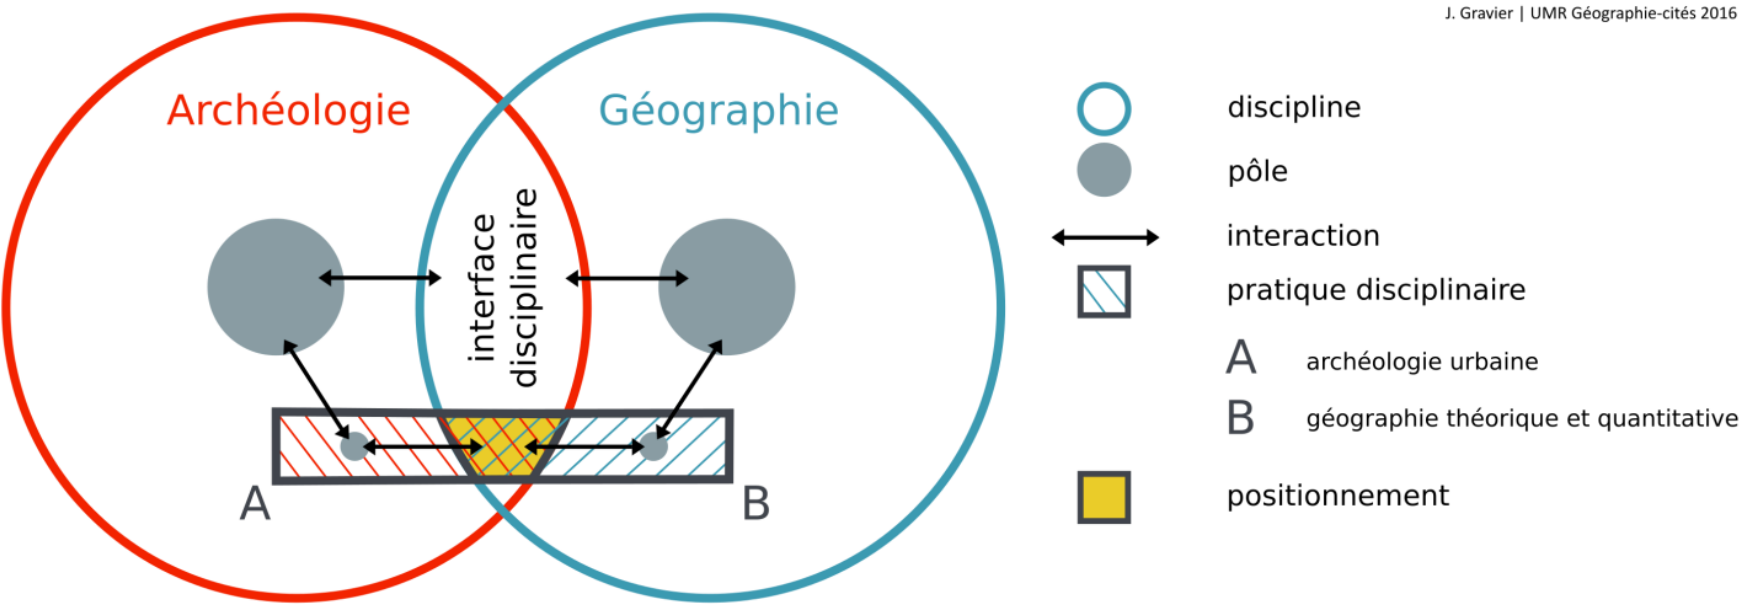
\includegraphics[width=\linewidth]{img/interfaces_disciplinaires_julie.png}
	\caption[Le \og positionnement d'interface disciplinaire entre l'archéologie urbaine et la géographie théorique et quantitative \fg{} de \textcite{gravier_deux_2018}]{Le \og positionnement d'interface disciplinaire entre l'archéologie urbaine et la géographie théorique et quantitative \fg{} de \textcite[fig. 1.3, \ppno~18]{gravier_deux_2018}.}
	\label{fig:interfaces-julie}
\end{figure}

Dans notre cas, c'est le modèle SimFeodal qui s'inscrit précisément dans cette même interface disciplinaire, et non l'un des chercheurs qui le co-construit.
En informatique, une interface peut aussi être un \og ensemble de règles, de conventions permettant un échange d’informations entre deux systèmes, deux éléments d’un système, ou entre l’utilisateur et la machine\fg{} \autocite{academie_francaise_interface_2019}.
La dernière définition est souvent employée, sous la forme \og d'interfaces utilisateur\fg{} (Interfaces Homme-Machine, IHM), qui peuvent notamment prendre une forme graphique, on parle alors d'interfaces graphiques ou, en anglais, de \og \textit{Graphical User Interface}\fg{} ou GUI.

Dans cette thèse, ces usages épistémologiques et informatiques se confondent.
SimFeodal est un modèle de simulation, un outil informatique, mais sa dimension collective et heuristique constitue une interface interdisciplinaire au sens épistémologique.
La démarche graphique mise en place, autour de l'évaluation visuelle, est bien une interface, c'est-à-dire une \og convention qui permet un échange\fg{}, pour reprendre la définition précédente \autocite{academie_francaise_interface_2019}, entre les utilisateurs.
Enfin, cette démarche est rendue possible par la création d'interfaces graphiques, au sens informatique, qui facilitent la visualisation des sorties du modèle, et permettent dès lors d'appréhender le modèle de manière exploratoire.


\paragraph{Une interface via la modélisation.}

L'une des conclusions du projet TransMonDyn est que la modélisation joue un rôle prépondérant d'incitation au dialogue entre thématiciens et modélisateurs.
La modélisation, au moins dans son aspect conceptuel ou ontologique (voir \cref{fig:ontologie-mediateur}), est en effet reconnue comme un facteur d'explicitation et donc de mise en place de connaissances communes :
\og C'est l'interaction entre les thématiciens et les modélisateurs (le plus souvent un seul mais parfois deux ou trois) de chaque sous-groupe qui a été moteur dans la construction du modèle.
\textelp{}
L'approche ontologique, par l'explicitation qu'elle implique, joue un rôle de médiation et facilite les échanges entre thématiciens et modélisateurs \fg{} \autocite[458]{sanders_points_2017}.

\begin{figure}[H]
	\centering
	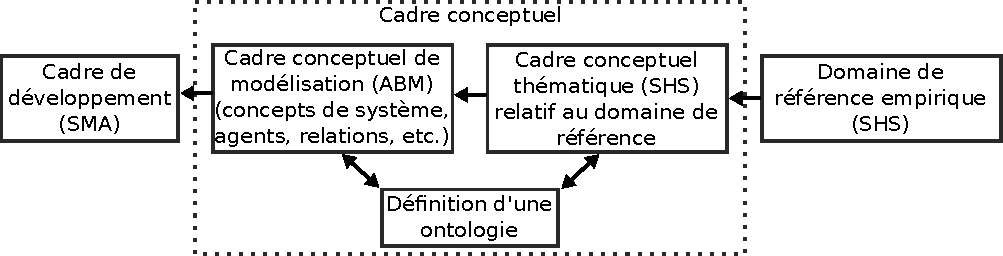
\includegraphics[width=\linewidth]{img/schema_phan.pdf}
	\caption[\og L'ontologie comme médiateur d'un dialogue \fg{} de \textcite{phan_ontologies_2014}]{\og L'ontologie comme médiateur d'un dialogue \fg{} de \textcite[fig. 2.7, \ppno~68]{phan_ontologies_2014}.}
	\label{fig:ontologie-mediateur}
\end{figure}

Il me semble que l'on peut aller plus loin dans ce raisonnement, et le généraliser à tous les domaines du modèle, et donc aussi à l'implémentation sous forme de modèle de simulation.
L'explicitation des connaissances est en effet une nécessité pour parvenir au modèle conceptuel, mais elle me semble encore plus importante lors du développement :
	dans un programme informatique, il ne peut y avoir aucune place au flou parce que l'ordinateur exécute sans chercher à interpréter.
Les lignes de code-source sont à ce titre un formalisme non ambigu, elles expriment précisément ce que la plateforme de simulation exécutera.
L'étape d'implémentation, qui aboutit sur un modèle de simulation, force donc plus encore que la modélisation conceptuelle à expliciter tous les choix effectués dans la modélisation.

Les quelque 2 500 lignes de code qui définissent le fonctionnement de SimFeodal ne sont pas exemptes de bugs ou d'erreurs d'implémentation, mais chacune d'elles répond à l'obligation de trancher la manière dont un mécanisme fonctionne.
Chacune de ces lignes entérine l'explicitation, par la formalisation informatique, des entités et interactions du modèle.
En cela, le développement d'un modèle de simulation émanant du modèle conceptuel constitue un apport qui ne se restreint pas à la possibilité de validation ou d'utilisation effective (à but prédictif par exemple) du modèle.
L'implémentation permet surtout de prolonger et renforcer l'explicitation, pousse à l'échange interdisciplinaire, et à ce titre, constitue aussi une méthode qui sert d'interface interdisciplinaire.

\paragraph{Une interface via la visualisation.}

Dans cette thèse, nous mettons en place une approche basée sur la représentation graphique et l'exploration visuelle, qui est employée tout au long du cycle de construction du modèle.
Le modèle est évalué en menant une analyse visuelle des sorties de simulation au travers des indicateurs de sortie majoritairement graphiques.
La comparaison entre différentes versions du modèle se fait aussi par le biais d'une comparaison visuelle entre les sorties correspondantes.
La sensibilité du modèle, enfin, est elle aussi analysée de manière visuelle, au moyen de représentations de la variabilité des indicateurs de sortie en fonction des réplications et valeurs de paramètres choisies.

De manière générale, je défends l'idée que les apports de la modélisation comme outil d'interdisciplinarité s'appliquent tout autant à la visualisation\footnote{
	Cette position est explicitée et détaillée dans \textcite{cura_visualisation_2020}.
}.
Comme la modélisation à base d'agents, la visualisation est un \og langage\fg{} compréhensible par le plus grand nombre, ne reposant pas sur un formalisme mathématique parfois excluant.
Comme la modélisation, la réalisation d'une représentation graphique pousse à l'explicitation de ce qui est représenté, de l'origine et des particularités des données mobilisées.
Comme la modélisation, la visualisation permet ainsi de créer une interface interdisciplinaire -- la représentation graphique d'un ensemble de données -- qui favorise alors le dialogue interdisciplinaire en le provoquant autour d'un élément accessible à tous les participants à un projet.

Pour ces raisons, les indicateurs de sortie de SimFeodal, les représentations graphiques permettant l'analyse de la sensibilité du modèle, ou encore, plus largement, SimEDB, la plateforme d'exploration des données issues de simulation, remplissent tous le rôle d'interface entre les disciplines du projet.
Ces interfaces permettent aux géographes, archéologues et historiens de dialoguer autour de représentations explicites, accessibles et intelligibles.


\paragraph{Une interface via l'exploration.}

Un dernier aspect de la démarche d'ensemble choisie pour ce travail de thèse me paraît en mesure de favoriser l'interdisciplinarité, en constituant une nouvelle interface disciplinaire.
Il s'agit de la nature fondamentalement exploratoire du processus (de co-construction et d'évaluation collective du modèle) mis en œuvre dans cette recherche.
La sous-partie suivante du chapitre détaille cette approche, mais on peut déjà en exprimer l'intérêt dans un cadre interdisciplinaire.

L'approche exploratoire, qu'elle soit inscrite dans l'analyse de données statistiques\footnote{
On parle alors d'\textit{Exploratory Data Analysis} ou \og EDA\fg{}, d'après \textcite{tukey_exploratory_1977}.
}, spatiales\footnote{
\textit{Exploratory Spatial Data Analysis}, \og ESDA\fg{}, d'après \textcites{brunsdon_exploratory_1998,haining_exploratory_1998}.
}, ou encore spatio-temporelles\footnote{
	On retrouve notamment cette approche, de manière très interactive, dans le champ des \textit{geovisual analytics} \autocite{andrienko_exploratory_2006}.
} permet de favoriser un raisonnement abductif \autocite{banos2005voie}.
Pour \citeauthor{yu_abduction_1994} (\citeyear{yu_abduction_1994}, in \textcite[2]{banos2005voie}) l'abduction désigne la \og capacité de l'être humain à générer des hypothèses temporaires à partir de l'information qu'il reçoit\fg{}.
En tant que position scientifique, \textcite[2]{banos2005voie} interprète l'abduction comme \og la capacité du scientifique à se mettre en position d’étonnement, à se laisser guider par la recherche de l'inattendu\fg{}.

L'abduction est très liée à l'analyse exploratoire de données, car fortement liée à la logique exploratoire : le raisonnement abductif survient quand on accepte de raisonner sur la seule base des données disponibles, sans chercher à les interpréter en fonction d'hypothèses pré-conçues auparavant.

La modélisation peut être guidée ou influencée par un principe d'abduction \autocite[77]{banos_pour_2013}, d'autant plus quand elle s'inscrit dans une logique exploratoire, acceptant là aussi de se fier \og uniquement\fg{} au modèle sans chercher forcément à interpréter ses écarts à la situation empirique comme des erreurs qui devraient être corrigées.

\textcite{morin1994interdisciplinarite} note qu'une approche abductive, par \og l'invention d'hypothèses explicatives nouvelles\fg{}, peut créer \og des articulations, organisatrices ou structurelles, entre des disciplines séparées et [permettre] de concevoir l'unité de ce qui était alors disjoint\fg{}.

L'approche exploratoire que nous entretenons dans ce travail collectif, en favorisant l'abduction, va aussi dans le sens d'une facilitation de l'interdisciplinarité.
Cette approche de modélisation exploratoire constitue dès lors, elle aussi, une interface disciplinaire : il s'agit bien d'une limite commune à l'archéologie et à la géographie qui permet les échanges entre ces disciplines\footnote{
	Pour paraphraser les termes de la définition du \textsc{Larousse} donnée plus haut.
}.
Elle permet d'oublier, par moments, les \textit{a priori} disciplinaires sur les causes de tel ou tel processus spatio-temporel, pour en proposer de nouvelles interprétations issues du modèle, de son exploration, et des discussions collectives entretenues autour de cette exploration.

\subsection{Une démarche exploratoire}

Dans la dernière sous-partie, je mentionnais l'intérêt d'une démarche exploratoire en ce qu'elle favorise l'abduction et donc l'interdisciplinarité.
De manière plus générale, l'approche exploratoire est essentielle au raisonnement tenu tout au long de ce travail de thèse.
Elle est ainsi mobilisée lors de chacune des étapes de la co-construction et de l'évaluation de SimFeodal, et constitue à chaque fois l'approche principalement suivie.
Dans cette dernière partie de définition du positionnement de ce travail de thèse, il me paraît important de préciser la manière dont cette démarche exploratoire s'exprime dans cette expérience de modélisation interdisciplinaire.

\paragraph{Un modèle exploratoire.}

Les archéologues, en particulier dans le monde anglophone, font emploi de la simulation informatique depuis le début des années 1970.
Parmi les chercheurs qui ont cherché à en décrire et à en catégoriser les usages, \citeauthor{mithen2018simulating} propose une typologie des modèles de simulation selon leurs buts.
Il distingue trois types de modèles de simulation, selon\footnote{
	\citeauthor{mithen2018simulating} \mkbibparens{\cite*{mithen2018simulating}, pp.~176--177; cité par \cite[260]{lake_trends_2014}}.
} :
\begin{compactenum}\vspace*{-0.5em}
	\item qu'ils servent à tester des hypothèses ;
	\item qu'ils aient pour but d'accompagner la construction théorique ;
	\item qu'ils soient conçus pour épauler le développement de nouvelles méthodes.
\end{compactenum}\vspace*{-0.5em}

Ce troisième type me paraît plus distant de notre usage, l'objectif de SimFeodal n'étant pas de proposer des méthodes innovantes dans le champ de la modélisation à base d'agents.
Au contraire, les objectifs de SimFeodal l'inscrivent tout à fait dans les deux premiers types, que \citeauthor{lake_trends_2014} explicite ainsi :
\begin{quotation}
\noindent \og 
When simulation models are used to test hypotheses the aim is usually to determine what actually happened in the past by comparing the output of a simulated process against the archaeological evidence.
In contrast, the use of simulation models to support theory building -- so-called heuristic modelling -- does not necessarily, or even usually, involve detailed comparison of output against the archaeological record;
in this case the purpose is not to test what happened in the past, but rather to understand how certain processes work and what sort of changes could plausibly have occurred.\\
\textelp{} \\
~[It] is important to recognise that the distinction between hypothesis-testing and theory-building simulation as conceived by Mithen is not always so clear cut in practice.
%On the one hand, comparing simulation output with archaeological evidence can ultimately contribute to theory building (e.g. Kohler and Varien 2012), while on the other hand simulation can be used to directly test hypothesis which are more about possible processes (e.g. the effect of parameters on model dynamics) than about what actually happened in the past (see Premo 2010, pp. 29–30).
\fg{} \\
\citetrackerfalse
\mbox{}~ \hfill \cite[260]{lake_trends_2014}
\citetrackertrue
\end{quotation}

À mon sens, SimFeodal s'inscrit précisément dans le cas identifié où la distinction entre ces deux approches n'est pas tranchée.
La conception du modèle s'appuie ainsi autant sur des théories que sur des données empiriques, en un continuum que nous appelons \og connaissance experte\fg{}.
Il s'agit bien de tester des hypothèses, mais sans nécessairement comparer les sorties du modèle à des données empiriques.
Cette confrontation de données empiriques et simulées est d'autant moins adaptée dans notre cas que les données empiriques sont très hétérogènes et lacunaires.

L'usage principal du modèle est donc expérimental.
On cherche bien à explorer les résultats d'interactions complexes entre agents, entre comportements pour accompagner la construction théorique.
On cherche toutefois tout autant à expérimenter les structures et processus que le modèle fait émerger, potentiellement sous l'influence de \og scénarios thématiques\fg{}, ce qui nous permet de tester des hypothèses.
Finalement, le modèle sert surtout de support au dialogue collectif et interdisciplinaire, mais il permet aussi, individuellement, pour chacun des participants, de repenser ou réorganiser la compréhension de la transition étudiée et des processus spatiaux modélisés.
En cela, c'est l'expérience de modélisation de SimFeodal, plus encore que le modèle en lui-même, qui se révèle intrinsèquement exploratoire.

\paragraph{Construit de manière exploratoire.}

La manière dont SimFeodal a été conçu, implémenté puis paramétré, pourrait sembler proche du \og bricolage\fg{} à certains modélisateurs expérimentés.
Par exemple, le fait que certains indicateurs de sortie de simulation -- ou pire, de mécanismes -- aient évolué au cours de la vie du modèle peut sembler caractéristique d'un modèle conceptuel défectueux ou incomplètement conçu.

Je souhaite au contraire défendre ce choix de modélisation, dans lequel priment les itérations entre le modèle, les résultats qu'il produit et les connaissances expertes sur lesquelles il s'appuie.
Dans ce mode de développement, tout élément du modèle implémenté peut être amené à évoluer, faisant alors évoluer l'élément équivalent dans le modèle conceptuel.
Si l'exploration du comportement du modèle montre qu'un type d'agent est peu utile, ou au contraire, qu'il serait judicieux de mieux distinguer des sous-types d'agents et de les doter de mécanismes propres, alors nous adapterons le modèle conceptuel.
Si les thématiciens, à l'occasion de nouvelles lectures, décident que le modèle conceptuel doit être modifié, alors il sera changé et donnera lieu à une nouvelle implémentation.
Ce aller-retour constant, où l'on accepte que les éléments, conceptuels ou implémentés, sont susceptibles de changer permet au fur et à mesure de consolider ou d'invalider la représentation que l'on a du système modélisé.

Cela rend la démarche de construction de SimFeodal profondément exploratoire :
dans une construction \og en spirale\fg{} \autocite[157]{mathian_objets_2014}, ce sont les connaissances acquises au travers de la modélisation qui guident la suite du processus de modélisation, et non directement les données empiriques ou la théorie initiale.
SimFeodal est donc un modèle que l'on pourrait qualifier d'\og auto-construit\fg{} -- en référence à l'auto-organisation --, l'expérience exploratoire de sa construction influant sur sa forme finale de manière performative.

\paragraph{Évalué et analysé de manière exploratoire.}
De manière plus classique, l'approche exploratoire est enfin appliquée aux données de sortie du modèle, selon le cadre méthodologique déjà mentionné de l'analyse exploratoire de données (EDA).
L'impermanence des indicateurs de sortie (cf. \hl{encadré incrémentalité indicateur}) en est une conséquence directe.
C'est en menant des analyses de ces indicateurs que l'on peut réaliser leurs défauts, ou leur incapacité parfois à départager.
C'est aussi en menant ces analyses que l'on peut constater le besoin de créer de nouveaux indicateurs, qui donneront une vision plus précise, ou légèrement différente, d'un phénomène quelconque.

Dans l'EDA, ce sont les données -- et les motifs qui en surgissent -- qui guident l'analyse et orientent vers l'étude de variantes ou transformations de ces mêmes données (normalisation des données, transformation en logarithmes, etc.).
Dans l'exploration de SimFeodal, ces \og données\fg{}, c'est-à-dire les indicateurs de sortie, guident elles-aussi l'évaluation du modèle, et leur étude entraîne de par là même des transformations de ces indicateurs (précision, distinction de catégories, changement de la méthode de calcul, etc.).

Dans l'approche classique, la visualisation n'est mobilisée qu'au début du processus d'évaluation, lors de la phase de \og \textit{face validation}\fg{}.
L'approche proposée dans cette thèse, nommée \og évaluation visuelle\fg{} (\hl{ref vers chapitre 3}), accorde au contraire un rôle clé à la visualisation tout au long du processus d'évaluation.
Les indicateurs de sortie sur lesquels on se base pour évaluer le modèle sont potentiellement classiques, mais le choix de faire reposer l'évaluation uniquement sur l'analyse visuelle de ces indicateurs me semble quant à elle assez hétérodoxe et profondément exploratoire.

De manière globale, c'est toute l'exploration du modèle qui a été menée de manière visuelle, en faisant appel à une plateforme -- SimEDB -- qui, comme les indicateurs et la méthode d'évaluation, a fortement évoluée tout au long de cette recherche.
Les \og résultats\fg{} du modèle, de même que sa sensibilité, n'ont pas été analysés au crible d'objectifs pré-définis stricts et hiérarchisés.
Les modalités de l'évaluation, telles que présentés dans ce manuscrit, résultent de nombreux allers-retours entre thématiciens et modélisateurs, et d'encore plus nombreux allers-retours entre le modèle et l'exploration, visuelle, de ses sorties.


\subsection{Une démarche reproductible}

La démarche d'ensemble poursuivie dans cette thèse est très exploratoire, et l'ensemble de ses composants ou étapes ont largement évolué durant les six années de cette expérience de co-construction interdisciplinaire.
Pour autant, afin que cette expérience puisse avoir une portée supérieure à celle d'un projet ponctuel, nous avons collectivement porté attention à lui garantir une certaine reproductibilité.
L'objectif, ce faisant, était que le modèle mis en place, et la démarche liée, puissent servir à d'autres chercheurs, notamment en histoire, en archéologie, en géographie, et de manière plus générale aux chercheurs s'intéressant à des phénomènes se déroulant sur de longues périodes temporelles.
Ceci afin d'accompagner ces chercheurs, à leur tour vers la modélisation de processus spatio-temporels sur le temps long.
Dans les paragraphes suivants, je détaille les méthodes mises en places dans ce projet pour appuyer la reproductibilité technique, méthodologique et conceptuelle de l'approche de co-construction de SimFeodal.

\paragraph{Réplicabilité technique.}

\textcite{reycoyrehourcq:hal-01677950} différencient reproductibilité, répétabilité et réplicabilité en ces termes :
\begin{quotation}
	\noindent \og
	Les définitions les plus courantes de ces notions sont ancrées dans le vocabulaire de la métrologie et des sciences computationnelles.
	Elles se rapportent donc au contrôle d'un ensemble de mesures.
	Dans le cas de la répétabilité, il s'agit d'effectuer des mesures répétées sur un même objet ou des objets similaires dans des conditions spécifiques.
	Dans un contexte de reproductibilité, ces mesures sont réalisées avec des instruments différents et dans des conditions variables (lieu, opérateur) qui doivent alors être spécifiées.
	La réplicabilité a été étudiée dans le domaine informatique et désigne la capacité de reproduire à l'identique les résultats d'une analyse.
	\fg{}\\
	\mbox{}~ \hfill \cite[411]{reycoyrehourcq:hal-01677950}
\end{quotation}

Nous avons veillé à garantir la \textbf{réplicabilité} de tout ce qui est décrit dans cette thèse en en partageant les sources.
Cela concerne bien sûr le modèle SimFeodal en lui-même\footnote{
\href{https://github.com/SimFeodal/SimFeodal}{https://github.com/SimFeodal/SimFeodal}
}, mais aussi les expériences qui ont été simulées\footnote{
	Dans le dossier \href{https://github.com/SimFeodal/SimFeodal/tree/master/experiments}{\textsf{/experiments/}} du dépôt de SimFeodal.
} et les outils permettant leur exploration\footnote{
\href{https://github.com/RCura/SimEDB}{https://github.com/RCura/SimEDB}
}.

À chaque fois que possible, les différentes versions des logiciels et \textit{packages} utilisés sont précisées dans les sources, et ce faisant, on approche ainsi d'une complétion de l'ensemble des \og paliers de réplicabilité\fg{} décrits dans la \cref{fig:paliers-replicabilite}.

\begin{figure}[H]
	\centering
	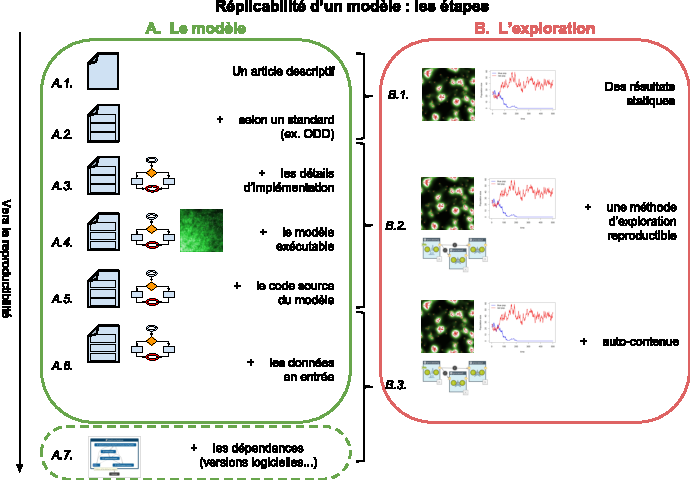
\includegraphics[width=\linewidth]{img/schema_reproductibilite.pdf}
	\caption[Les paliers de réplicabilité d’un modèle de simulation et de son exploration.]{\og Les paliers de réplicabilité d’un modèle de simulation et de son exploration \fg{} in \textcite[fig. 3, \ppno~427]{reycoyrehourcq:hal-01677950}.}
	\label{fig:paliers-replicabilite}
\end{figure}

Pour renforcer cette réplicabilité technique et lui donner une dimension universelle, c'est-à-dire pour que chacun puisse répliquer les expériences et résultats produits avec SimFeodal, nous avons de plus fait le choix, militant, de ne mobiliser que des outils sous licences libres.
C'est le cas de la plateforme de simulation Gama \autocite{taillandier_building_2018} avec laquelle SimFeodal a été conçue, c'est aussi le cas du langage de programmation R \autocite{r_core_team_r_2019} utilisé pour toutes les analyses, de la base de données OmniSciDB utilisée dans la plate-forme d'exploration des données \autocite{root_mapd_2016}, et des outils utilisés pour construire cette plateforme \autocite[par exemple]{chang_shiny_2017}.

Au-delà des productions \og logicielles\fg{} liées à SimFeodal et à son exploration, notons que dans le cadre de ce manuscrit de thèse, les outils mobilisés sont eux aussi libres : ce manuscrit est rédigé avec \LaTeX, les figures ont été produites avec R\footnote{
	Les données et codes-sources en sont alors disponibles dans le dépôt logiciel de ce manuscrit.
} ou avec le logiciel libre de dessin vectoriel Inkscape, le tout en utilisant un système d'exploitation libre pour la rédaction comme pour l'exécution des simulations.

\paragraph{Reproductibilité méthodologique et conceptuelle.}

Les solutions techniques, et la publication de leurs sources, présentées dans ce travail de thèse garantissent une réplicabilité technique.
Cette dernière n'est pourtant qu'un des composants, et sans doute le plus simple, de la reproductibilité plus large que nous visons.

Nous souhaitons ainsi que l'expérience qui est la nôtre puisse servir ou inspirer d'autres projets, et avons pour cela tenté de communiquer autant que possible sur SimFeodal.
Ces communications, orales ou écrites, visaient différents publics, représentatifs des concepteurs du modèle.
Il s'agissait ainsi d'une part d'inspirer des archéologues et historiens à se lancer dans l'expérience de la modélisation, au moyen du paradigme des modèles à base d'agents qui nous semble porteur et accessible.
Pour que ces restitutions de notre travail trouvent une résonance, et donc une audience adaptée, elles ont été effectuées devant un public d'archéologues et d'historiens sensibles aux méthodes (Journées Informatique et Archéologies de Paris, Séminaire TransMonDyn à Washington State University, organisation en cours d'un séminaire de restitution à destination d'historiens).

Il s'agissait aussi de convaincre des chercheurs pratiquant déjà la modélisation de l'intérêt de l'étude des dynamiques spatiales sur le temps long, par exemple à travers des chapitres d'ouvrages interdisciplinaires \autocite{tannier_ontologie_2014,cura_transition_2017}, en ciblant notamment la communauté de la géographie théorique et quantitative, que ce soit à l'occasion de colloques (ThéoQuant 2015 et 2017, ECTQG 2015, 2017 et 2019) ou de journées d'études liées à d'autres projets de modélisation.

En dehors des publications et communications qui marquent des \og points d'étape\fg{} de la construction du modèle et de son exploration, nous avons fait le choix d'en \og versionner\fg{} l'évolution, dans un dépôt logiciel de versionnement adapté, afin que celle-ci puisse être retracée et analysée \textit{a posteriori}.
C'est aussi le cas de la plateforme d'exploration des sorties du modèle, SimEDB, dont le dépôt retrace l'ensemble des évolutions décrites dans le \hl{chapitre 5}.

De manière plus large, ce manuscrit s'inscrit dans la volonté de replacer le modèle SimFeodal dans le cadre plus large des modèles descriptifs, exploratoires et conçus dans un cadre interdisciplinaire.
Ces dépôts logiciels concourent à l'intention de retracer le raisonnement -- générique et spécifique -- qui a amené au modèle SimFeodal tel que présenté dans le \hl{chapitre 2}.
En cherchant à documenter les alternatives disponibles qui ont été rencontrées tout au long de la conception du modèle et de la plateforme d'exploration de ses sorties, en cherchant à justifier les choix effectués, qu'ils soient conceptuels (\hl{chapitres 2 et 3}), méthodologiques (\hl{chapitre 3, 5 et 6}) ou parfois techniques (\hl{chapitre 5}), en suivant des modes de descriptions standards (ODD pour le modèle, MCD pour la base de données), je suis convaincu d'accroître le potentiel de reproductibilité du modèle, et plus largement, de la démarche mise en place pour le construire et l'évaluer.

Cette thèse prend ainsi la forme d'un retour d'expérience, partial mais argumenté, et surtout documenté autant que possible.
L'ambition est d'ouvrir la voie à d'autres expériences de ce type et de tenter de convaincre de l'intérêt, pour les projets interdisciplinaires, tout à la fois, de la modélisation à base d'agents, d'une démarche de co-construction, et de la commodité des approches visuelles pour les accompagner.


\section*{Conclusion}
\addcontentsline{toc}{section}{\protect\numberline{}Conclusion}

Dans ce chapitre, j'ai essayé de préciser les objets étudiés dans ce travail de thèse, la manière de les étudier, et les raisons, contextuelles et liées à mon parcours personnel, qui ont conduit aux approches mises en place.

De manière générale, on peut résumer ces approches au moyen des quatre termes mis en exergue dans la dernière partie de ce chapitre.
Autour d'un objet de recherche constitué par la modélisation de dynamiques spatiales sur le temps long, dans un contexte interdisciplinaire, je défends ainsi une approche résolument ancrée dans la co-construction.
Celle-ci va plus loin que l'accompagnement dans l'interaction entre \og thématiciens\fg{} et \og modélisateurs\fg{} en cherchant autant que possible à faire prendre part, à chacun des participants de projet, à l'ensemble des étapes de conception, de construction et d'évaluation du modèle.
L'ambition n'est pas que chaque participant devienne expert dans chacune de ces étapes, mais que toutes les décisions adoptées dans de ces étapes soient collectives et justifiables par chacun.

La démarche de co-construction est facilitée par l'adoption d'une approche exploratoire de la modélisation.
Collectivement, nous ne cherchons pas à créer un modèle qui soit validable et utilisable, par exemple à but rétro-prédictif, mais au contraire à construire un modèle exploratoire, dont la construction et l'exploration en elles-mêmes sont les vecteurs d'acquisition de connaissance par les participants au projet.
En multipliant les allers-retours entre la conception, l'implémentation et l'évaluation du modèle, on adopte une position exploratoire qui s'inscrit dans une certaine visée abductive.

Pour que cette approche exploratoire puisse toutefois être mobilisée par d'autres et ne se cantonne pas à une expérimentation isolée, nous faisons le choix de documenter, pour en assurer la réplicabilité, toutes les productions informatiques mises en œuvre autour du modèle SimFeodal.
Pour aller plus loin, nous documentons aussi les nombreuses évolutions du modèle, de son évaluation et de son exploration, au sein d'outils de versionnement publics et au travers de disséminations académiques diversifiées de nos travaux.
On cherche ainsi à tendre vers la reproductibilité de la démarche mise en place, de manière à inscrire ce retour d'expérience dans un cadre de cumulativité des connaissances (\textcite{pumain_cumulativite_2005}, citée par \textcite{reycoyrehourcq:hal-01677950}, p.~431).

Ce faisant, j'espère positionner l'ensemble des travaux décrits dans cette thèse comme des instruments d'interface disciplinaires.
Les choix du paradigme de modélisation à base d'agents, d'une démarche de co-construction, de méthodes d'évaluation visuelles et interactives, sont, à mon sens, autant de solutions permettant de faciliter l'interdisciplinarité en s'inscrivant dans des domaines scientifiques accessibles et communs aux membres du projet.
Le modèle SimFeodal se situe à l'interface entre géographie et sciences historiques, la plateforme d'exploration SimEDB à l'interface entre modélisation en sciences sociales et informatique liée à l'interaction homme-machine.
Ces outils et les approches suivies pour leur construction participent au rôle d'interface de ce travail de thèse, et plus largement, de ce projet collectif et interdisciplinaire de modélisation.

Ma position personnelle n'est pas celle d'une interface -- je suis géographe, modélisateur, géomaticien -- mais celle d'un passeur, sélectionnant des outils et méthodes éprouvés dans chacune des communautés afin de les agencer et de les mettre au service d'un projet collectif.
